\documentclass[twoside]{book}

% Packages required by doxygen
\usepackage{fixltx2e}
\usepackage{calc}
\usepackage{doxygen}
\usepackage[export]{adjustbox} % also loads graphicx
\usepackage{graphicx}
\usepackage[utf8]{inputenc}
\usepackage{makeidx}
\usepackage{multicol}
\usepackage{multirow}
\PassOptionsToPackage{warn}{textcomp}
\usepackage{textcomp}
\usepackage[nointegrals]{wasysym}
\usepackage[table]{xcolor}

% Font selection
\usepackage[T1]{fontenc}
\usepackage[scaled=.90]{helvet}
\usepackage{courier}
\usepackage{amssymb}
\usepackage{sectsty}
\renewcommand{\familydefault}{\sfdefault}
\allsectionsfont{%
  \fontseries{bc}\selectfont%
  \color{darkgray}%
}
\renewcommand{\DoxyLabelFont}{%
  \fontseries{bc}\selectfont%
  \color{darkgray}%
}
\newcommand{\+}{\discretionary{\mbox{\scriptsize$\hookleftarrow$}}{}{}}

% Page & text layout
\usepackage{geometry}
\geometry{%
  a4paper,%
  top=2.5cm,%
  bottom=2.5cm,%
  left=2.5cm,%
  right=2.5cm%
}
\tolerance=750
\hfuzz=15pt
\hbadness=750
\setlength{\emergencystretch}{15pt}
\setlength{\parindent}{0cm}
\setlength{\parskip}{3ex plus 2ex minus 2ex}
\makeatletter
\renewcommand{\paragraph}{%
  \@startsection{paragraph}{4}{0ex}{-1.0ex}{1.0ex}{%
    \normalfont\normalsize\bfseries\SS@parafont%
  }%
}
\renewcommand{\subparagraph}{%
  \@startsection{subparagraph}{5}{0ex}{-1.0ex}{1.0ex}{%
    \normalfont\normalsize\bfseries\SS@subparafont%
  }%
}
\makeatother

% Headers & footers
\usepackage{fancyhdr}
\pagestyle{fancyplain}
\fancyhead[LE]{\fancyplain{}{\bfseries\thepage}}
\fancyhead[CE]{\fancyplain{}{}}
\fancyhead[RE]{\fancyplain{}{\bfseries\leftmark}}
\fancyhead[LO]{\fancyplain{}{\bfseries\rightmark}}
\fancyhead[CO]{\fancyplain{}{}}
\fancyhead[RO]{\fancyplain{}{\bfseries\thepage}}
\fancyfoot[LE]{\fancyplain{}{}}
\fancyfoot[CE]{\fancyplain{}{}}
\fancyfoot[RE]{\fancyplain{}{\bfseries\scriptsize Generated by Doxygen }}
\fancyfoot[LO]{\fancyplain{}{\bfseries\scriptsize Generated by Doxygen }}
\fancyfoot[CO]{\fancyplain{}{}}
\fancyfoot[RO]{\fancyplain{}{}}
\renewcommand{\footrulewidth}{0.4pt}
\renewcommand{\chaptermark}[1]{%
  \markboth{#1}{}%
}
\renewcommand{\sectionmark}[1]{%
  \markright{\thesection\ #1}%
}

% Indices & bibliography
\usepackage{natbib}
\usepackage[titles]{tocloft}
\setcounter{tocdepth}{3}
\setcounter{secnumdepth}{5}
\makeindex

% Hyperlinks (required, but should be loaded last)
\usepackage{ifpdf}
\ifpdf
  \usepackage[pdftex,pagebackref=true]{hyperref}
\else
  \usepackage[ps2pdf,pagebackref=true]{hyperref}
\fi
\hypersetup{%
  colorlinks=true,%
  linkcolor=blue,%
  citecolor=blue,%
  unicode%
}

% Custom commands
\newcommand{\clearemptydoublepage}{%
  \newpage{\pagestyle{empty}\cleardoublepage}%
}

\usepackage{caption}
\captionsetup{labelsep=space,justification=centering,font={bf},singlelinecheck=off,skip=4pt,position=top}

%===== C O N T E N T S =====

\begin{document}

% Titlepage & ToC
\hypersetup{pageanchor=false,
             bookmarksnumbered=true,
             pdfencoding=unicode
            }
\pagenumbering{alph}
\begin{titlepage}
\vspace*{7cm}
\begin{center}%
{\Large My Project }\\
\vspace*{1cm}
{\large Generated by Doxygen 1.8.13}\\
\end{center}
\end{titlepage}
\clearemptydoublepage
\pagenumbering{roman}
\tableofcontents
\clearemptydoublepage
\pagenumbering{arabic}
\hypersetup{pageanchor=true}

%--- Begin generated contents ---
\chapter{Hierarchical Index}
\section{Class Hierarchy}
This inheritance list is sorted roughly, but not completely, alphabetically\+:\begin{DoxyCompactList}
\item \contentsline{section}{Date}{\pageref{class_date}}{}
\item \contentsline{section}{Employee}{\pageref{class_employee}}{}
\item \contentsline{section}{Existing\+ID$<$ T $>$}{\pageref{class_existing_i_d}}{}
\item \contentsline{section}{Headquarters}{\pageref{class_headquarters}}{}
\item \contentsline{section}{I\+D\+Not\+Found$<$ T $>$}{\pageref{class_i_d_not_found}}{}
\item \contentsline{section}{Invalid\+Date$<$ T $>$}{\pageref{class_invalid_date}}{}
\item \contentsline{section}{Production\+\_\+\+Request}{\pageref{class_production___request}}{}
\item \contentsline{section}{Publication}{\pageref{class_publication}}{}
\begin{DoxyCompactList}
\item \contentsline{section}{Book}{\pageref{class_book}}{}
\item \contentsline{section}{Journal}{\pageref{class_journal}}{}
\end{DoxyCompactList}
\item \contentsline{section}{Store}{\pageref{class_store}}{}
\item \contentsline{section}{Store\+\_\+\+Request}{\pageref{class_store___request}}{}
\end{DoxyCompactList}

\chapter{Class Index}
\section{Class List}
Here are the classes, structs, unions and interfaces with brief descriptions\+:\begin{DoxyCompactList}
\item\contentsline{section}{\hyperlink{class_binary_node}{Binary\+Node$<$ Comparable $>$} }{\pageref{class_binary_node}}{}
\item\contentsline{section}{\hyperlink{class_book}{Book} \\*Class \hyperlink{class_book}{Book} -\/ creates the object \hyperlink{class_book}{Book} -\/ type of \hyperlink{class_publication}{Publication} }{\pageref{class_book}}{}
\item\contentsline{section}{\hyperlink{class_b_s_t}{B\+S\+T$<$ Comparable $>$} }{\pageref{class_b_s_t}}{}
\item\contentsline{section}{\hyperlink{class_b_s_t_itr_in}{B\+S\+T\+Itr\+In$<$ Comparable $>$} }{\pageref{class_b_s_t_itr_in}}{}
\item\contentsline{section}{\hyperlink{class_b_s_t_itr_level}{B\+S\+T\+Itr\+Level$<$ Comparable $>$} }{\pageref{class_b_s_t_itr_level}}{}
\item\contentsline{section}{\hyperlink{class_b_s_t_itr_post}{B\+S\+T\+Itr\+Post$<$ Comparable $>$} }{\pageref{class_b_s_t_itr_post}}{}
\item\contentsline{section}{\hyperlink{class_b_s_t_itr_pre}{B\+S\+T\+Itr\+Pre$<$ Comparable $>$} }{\pageref{class_b_s_t_itr_pre}}{}
\item\contentsline{section}{\hyperlink{class_date}{Date} \\*Class \hyperlink{class_date}{Date} -\/ Year / month / day }{\pageref{class_date}}{}
\item\contentsline{section}{\hyperlink{class_employee}{Employee} \\*Class \hyperlink{class_employee}{Employee} that creates an object (\hyperlink{class_employee}{Employee}) }{\pageref{class_employee}}{}
\item\contentsline{section}{\hyperlink{class_existing_i_d}{Existing\+I\+D$<$ T $>$} \\*Class \hyperlink{class_existing_i_d}{Existing\+ID} -\/ is a Template$<$\+Class T$>$ exception }{\pageref{class_existing_i_d}}{}
\item\contentsline{section}{\hyperlink{class_headquarters}{Headquarters} \\*Class \hyperlink{class_headquarters}{Headquarters} the main class that contains everything (support where the company works) }{\pageref{class_headquarters}}{}
\item\contentsline{section}{\hyperlink{class_i_d_not_found}{I\+D\+Not\+Found$<$ T $>$} \\*Class \hyperlink{class_i_d_not_found}{I\+D\+Not\+Found} -\/ is a Template$<$\+Class T$>$ exception }{\pageref{class_i_d_not_found}}{}
\item\contentsline{section}{\hyperlink{class_invalid_date}{Invalid\+Date$<$ T $>$} \\*Class \hyperlink{class_invalid_date}{Invalid\+Date} -\/ is a Template$<$\+Class T$>$ exception }{\pageref{class_invalid_date}}{}
\item\contentsline{section}{\hyperlink{class_journal}{Journal} \\*Class \hyperlink{class_journal}{Journal} -\/ creates the object \hyperlink{class_journal}{Journal} -\/ type of \hyperlink{class_publication}{Publication} }{\pageref{class_journal}}{}
\item\contentsline{section}{\hyperlink{class_production___request}{Production\+\_\+\+Request} \\*Class Production request to be done by \hyperlink{class_headquarters}{Headquarters} }{\pageref{class_production___request}}{}
\item\contentsline{section}{\hyperlink{class_publication}{Publication} \\*Class \hyperlink{class_publication}{Publication}, abstract, Class parent of \hyperlink{class_book}{Book} and \hyperlink{class_journal}{Journal} }{\pageref{class_publication}}{}
\item\contentsline{section}{\hyperlink{class_store}{Store} \\*Class \hyperlink{class_store}{Store} -\/ creates an object \hyperlink{class_store}{Store} }{\pageref{class_store}}{}
\item\contentsline{section}{\hyperlink{class_store___request}{Store\+\_\+\+Request} \\*Class \hyperlink{class_store___request}{Store\+\_\+\+Request} to save the requests of the stores to be completed by \hyperlink{class_headquarters}{Headquarters} }{\pageref{class_store___request}}{}
\item\contentsline{section}{\hyperlink{structsuspencion_hash}{suspencion\+Hash} }{\pageref{structsuspencion_hash}}{}
\item\contentsline{section}{\hyperlink{class_suspended___request}{Suspended\+\_\+\+Request} \\*Class \hyperlink{class_suspended___request}{Suspended\+\_\+\+Request} }{\pageref{class_suspended___request}}{}
\end{DoxyCompactList}

\chapter{Class Documentation}
\hypertarget{class_book}{}\section{Book Class Reference}
\label{class_book}\index{Book@{Book}}


Class \hyperlink{class_book}{Book} -\/ creates the object \hyperlink{class_book}{Book} -\/ type of \hyperlink{class_publication}{Publication}.  




{\ttfamily \#include $<$Book.\+h$>$}

Inheritance diagram for Book\+:\begin{figure}[H]
\begin{center}
\leavevmode
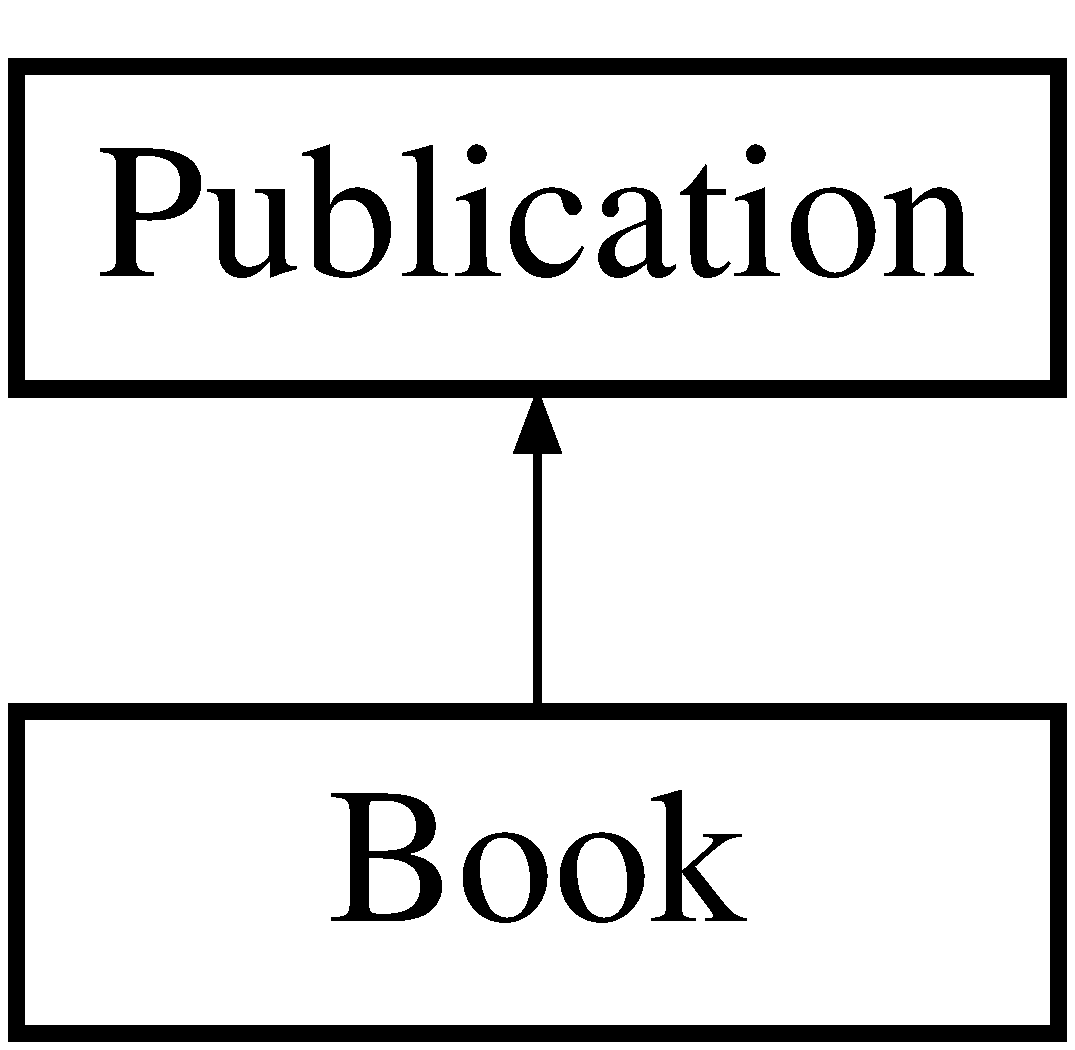
\includegraphics[height=2.000000cm]{class_book}
\end{center}
\end{figure}
\subsection*{Public Member Functions}
\begin{DoxyCompactItemize}
\item 
\hyperlink{class_book_a45ca53a239ae4614d7cc687a07a5c96e}{Book} (int id, std\+::string desc, std\+::string col)
\begin{DoxyCompactList}\small\item\em \hyperlink{class_book}{Book} Default constructor. \end{DoxyCompactList}\item 
void \hyperlink{class_book_a8368f243d8a645444e8019760a50cc8b}{show} ()
\begin{DoxyCompactList}\small\item\em Displays the information of the book (his parameters) \end{DoxyCompactList}\item 
std\+::string \hyperlink{class_book_ab72570b8b4d902d6f3fe681dc29b2198}{get\+Out\+Put} (int type)
\begin{DoxyCompactList}\small\item\em Gets the output to be written to the file. \end{DoxyCompactList}\item 
int \hyperlink{class_book_a285dd3654bfced6baffd86320c39d42e}{get\+Type} () const
\begin{DoxyCompactList}\small\item\em Gets the type of the book. \end{DoxyCompactList}\end{DoxyCompactItemize}
\subsection*{Additional Inherited Members}


\subsection{Detailed Description}
Class \hyperlink{class_book}{Book} -\/ creates the object \hyperlink{class_book}{Book} -\/ type of \hyperlink{class_publication}{Publication}. 

\subsection{Constructor \& Destructor Documentation}
\mbox{\Hypertarget{class_book_a45ca53a239ae4614d7cc687a07a5c96e}\label{class_book_a45ca53a239ae4614d7cc687a07a5c96e}} 
\index{Book@{Book}!Book@{Book}}
\index{Book@{Book}!Book@{Book}}
\subsubsection{\texorpdfstring{Book()}{Book()}}
{\footnotesize\ttfamily Book\+::\+Book (\begin{DoxyParamCaption}\item[{int}]{id,  }\item[{std\+::string}]{desc,  }\item[{std\+::string}]{col }\end{DoxyParamCaption})}



\hyperlink{class_book}{Book} Default constructor. 


\begin{DoxyParams}{Parameters}
{\em id} & unique way to identify all the books \\
\hline
{\em desc} & description of the book \\
\hline
{\em col} & collecting of the book \\
\hline
\end{DoxyParams}


\subsection{Member Function Documentation}
\mbox{\Hypertarget{class_book_ab72570b8b4d902d6f3fe681dc29b2198}\label{class_book_ab72570b8b4d902d6f3fe681dc29b2198}} 
\index{Book@{Book}!get\+Out\+Put@{get\+Out\+Put}}
\index{get\+Out\+Put@{get\+Out\+Put}!Book@{Book}}
\subsubsection{\texorpdfstring{get\+Out\+Put()}{getOutPut()}}
{\footnotesize\ttfamily string Book\+::get\+Out\+Put (\begin{DoxyParamCaption}\item[{int}]{type }\end{DoxyParamCaption})\hspace{0.3cm}{\ttfamily [virtual]}}



Gets the output to be written to the file. 


\begin{DoxyParams}{Parameters}
{\em type} & of the publication as an int value, 0 if book and 1 if journal\\
\hline
\end{DoxyParams}
\begin{DoxyReturn}{Returns}
the string to write to the file 
\end{DoxyReturn}


Reimplemented from \hyperlink{class_publication_af382f9557807e8375478ceb7890e841f}{Publication}.

\mbox{\Hypertarget{class_book_a285dd3654bfced6baffd86320c39d42e}\label{class_book_a285dd3654bfced6baffd86320c39d42e}} 
\index{Book@{Book}!get\+Type@{get\+Type}}
\index{get\+Type@{get\+Type}!Book@{Book}}
\subsubsection{\texorpdfstring{get\+Type()}{getType()}}
{\footnotesize\ttfamily int Book\+::get\+Type (\begin{DoxyParamCaption}{ }\end{DoxyParamCaption}) const\hspace{0.3cm}{\ttfamily [virtual]}}



Gets the type of the book. 

\begin{DoxyReturn}{Returns}
int value which is the type of the publication, 0 if book and 1 if journal 
\end{DoxyReturn}


Reimplemented from \hyperlink{class_publication_ab0bd9119b29b09fbbe9044016a512407}{Publication}.

\mbox{\Hypertarget{class_book_a8368f243d8a645444e8019760a50cc8b}\label{class_book_a8368f243d8a645444e8019760a50cc8b}} 
\index{Book@{Book}!show@{show}}
\index{show@{show}!Book@{Book}}
\subsubsection{\texorpdfstring{show()}{show()}}
{\footnotesize\ttfamily void Book\+::show (\begin{DoxyParamCaption}{ }\end{DoxyParamCaption})\hspace{0.3cm}{\ttfamily [virtual]}}



Displays the information of the book (his parameters) 

\begin{DoxyReturn}{Returns}
void 
\end{DoxyReturn}


Reimplemented from \hyperlink{class_publication_aa4240a04fcecd6257e0d1a33e8f18ff0}{Publication}.



The documentation for this class was generated from the following files\+:\begin{DoxyCompactItemize}
\item 
Book.\+h\item 
Book.\+cpp\end{DoxyCompactItemize}

\hypertarget{class_date}{}\section{Date Class Reference}
\label{class_date}\index{Date@{Date}}


Class \hyperlink{class_date}{Date} -\/ Year / month / day.  




{\ttfamily \#include $<$Date.\+h$>$}

\subsection*{Public Member Functions}
\begin{DoxyCompactItemize}
\item 
\hyperlink{class_date_a818cdeae426d62baca78fb24a3041395}{Date} (unsigned int y, unsigned int m, unsigned int d)
\begin{DoxyCompactList}\small\item\em Default constructor. \end{DoxyCompactList}\item 
void \hyperlink{class_date_a12214ddd7d5aa3d614d8a068b9701bc4}{set\+Year} (unsigned int y)
\begin{DoxyCompactList}\small\item\em Changes the year of the \hyperlink{class_date}{Date}. \end{DoxyCompactList}\item 
void \hyperlink{class_date_ab2c14958d6ac7b88f37e741e82e456db}{set\+Month} (unsigned int m)
\begin{DoxyCompactList}\small\item\em Changes the month of the \hyperlink{class_date}{Date}. \end{DoxyCompactList}\item 
void \hyperlink{class_date_ad0d7be5956f115287e09fd31d4f91fad}{set\+Day} (unsigned int d)
\begin{DoxyCompactList}\small\item\em Changes the day of \hyperlink{class_date}{Date}. \end{DoxyCompactList}\item 
void \hyperlink{class_date_a81c1ecac7b2fe04d586097866481e830}{set\+Date} (unsigned int y, unsigned int m, unsigned int d)
\begin{DoxyCompactList}\small\item\em Changes the \hyperlink{class_date}{Date}. \end{DoxyCompactList}\item 
unsigned int \hyperlink{class_date_a597b505c264a24d34369c43119fc4e6e}{get\+Year} () const
\begin{DoxyCompactList}\small\item\em Gets the year of the \hyperlink{class_date}{Date}. \end{DoxyCompactList}\item 
unsigned int \hyperlink{class_date_a6152596dcf2e1e78e2095ea518de59e7}{get\+Month} () const
\begin{DoxyCompactList}\small\item\em Gets the month of the \hyperlink{class_date}{Date}. \end{DoxyCompactList}\item 
unsigned int \hyperlink{class_date_a13855b25efb79eaf7dccf08555421a1d}{get\+Day} () const
\begin{DoxyCompactList}\small\item\em Gets the day of the \hyperlink{class_date}{Date}. \end{DoxyCompactList}\item 
void \hyperlink{class_date_addaed921af229dffeb35ef7ef30bff29}{show} ()
\begin{DoxyCompactList}\small\item\em Shows the date on the screen in format \char`\"{}yyyy/mm/dd\char`\"{}. \end{DoxyCompactList}\item 
bool \hyperlink{class_date_a09704874041e417655bf7be43596da80}{operator$<$} (const \hyperlink{class_date}{Date} \&d2) const
\begin{DoxyCompactList}\small\item\em operator $<$ for the \hyperlink{class_date}{Date} \end{DoxyCompactList}\item 
bool \hyperlink{class_date_ab33fabb71e001e3bb98aa3aff846ea65}{operator==} (const \hyperlink{class_date}{Date} \&d2) const
\begin{DoxyCompactList}\small\item\em operator == for the \hyperlink{class_date}{Date} \end{DoxyCompactList}\end{DoxyCompactItemize}


\subsection{Detailed Description}
Class \hyperlink{class_date}{Date} -\/ Year / month / day. 

\subsection{Constructor \& Destructor Documentation}
\mbox{\Hypertarget{class_date_a818cdeae426d62baca78fb24a3041395}\label{class_date_a818cdeae426d62baca78fb24a3041395}} 
\index{Date@{Date}!Date@{Date}}
\index{Date@{Date}!Date@{Date}}
\subsubsection{\texorpdfstring{Date()}{Date()}}
{\footnotesize\ttfamily Date\+::\+Date (\begin{DoxyParamCaption}\item[{unsigned int}]{y,  }\item[{unsigned int}]{m,  }\item[{unsigned int}]{d }\end{DoxyParamCaption})}



Default constructor. 


\begin{DoxyParams}{Parameters}
{\em y} & year of the \hyperlink{class_date}{Date} \\
\hline
{\em m} & month of the \hyperlink{class_date}{Date} \\
\hline
{\em d} & day of the \hyperlink{class_date}{Date} \\
\hline
\end{DoxyParams}


\subsection{Member Function Documentation}
\mbox{\Hypertarget{class_date_a13855b25efb79eaf7dccf08555421a1d}\label{class_date_a13855b25efb79eaf7dccf08555421a1d}} 
\index{Date@{Date}!get\+Day@{get\+Day}}
\index{get\+Day@{get\+Day}!Date@{Date}}
\subsubsection{\texorpdfstring{get\+Day()}{getDay()}}
{\footnotesize\ttfamily unsigned int Date\+::get\+Day (\begin{DoxyParamCaption}{ }\end{DoxyParamCaption}) const}



Gets the day of the \hyperlink{class_date}{Date}. 

\begin{DoxyReturn}{Returns}
day of the \hyperlink{class_date}{Date} 
\end{DoxyReturn}
\mbox{\Hypertarget{class_date_a6152596dcf2e1e78e2095ea518de59e7}\label{class_date_a6152596dcf2e1e78e2095ea518de59e7}} 
\index{Date@{Date}!get\+Month@{get\+Month}}
\index{get\+Month@{get\+Month}!Date@{Date}}
\subsubsection{\texorpdfstring{get\+Month()}{getMonth()}}
{\footnotesize\ttfamily unsigned int Date\+::get\+Month (\begin{DoxyParamCaption}{ }\end{DoxyParamCaption}) const}



Gets the month of the \hyperlink{class_date}{Date}. 

\begin{DoxyReturn}{Returns}
month of the \hyperlink{class_date}{Date} 
\end{DoxyReturn}
\mbox{\Hypertarget{class_date_a597b505c264a24d34369c43119fc4e6e}\label{class_date_a597b505c264a24d34369c43119fc4e6e}} 
\index{Date@{Date}!get\+Year@{get\+Year}}
\index{get\+Year@{get\+Year}!Date@{Date}}
\subsubsection{\texorpdfstring{get\+Year()}{getYear()}}
{\footnotesize\ttfamily unsigned int Date\+::get\+Year (\begin{DoxyParamCaption}{ }\end{DoxyParamCaption}) const}



Gets the year of the \hyperlink{class_date}{Date}. 

\begin{DoxyReturn}{Returns}
year of the \hyperlink{class_date}{Date} 
\end{DoxyReturn}
\mbox{\Hypertarget{class_date_a09704874041e417655bf7be43596da80}\label{class_date_a09704874041e417655bf7be43596da80}} 
\index{Date@{Date}!operator$<$@{operator$<$}}
\index{operator$<$@{operator$<$}!Date@{Date}}
\subsubsection{\texorpdfstring{operator$<$()}{operator<()}}
{\footnotesize\ttfamily bool Date\+::operator$<$ (\begin{DoxyParamCaption}\item[{const \hyperlink{class_date}{Date} \&}]{d2 }\end{DoxyParamCaption}) const}



operator $<$ for the \hyperlink{class_date}{Date} 


\begin{DoxyParams}{Parameters}
{\em d2} & \hyperlink{class_date}{Date} d2 to the compared\\
\hline
\end{DoxyParams}
\begin{DoxyReturn}{Returns}
true if \char`\"{}\+Date $<$ d2\char`\"{} and false otherwise 
\end{DoxyReturn}
\mbox{\Hypertarget{class_date_ab33fabb71e001e3bb98aa3aff846ea65}\label{class_date_ab33fabb71e001e3bb98aa3aff846ea65}} 
\index{Date@{Date}!operator==@{operator==}}
\index{operator==@{operator==}!Date@{Date}}
\subsubsection{\texorpdfstring{operator==()}{operator==()}}
{\footnotesize\ttfamily bool Date\+::operator== (\begin{DoxyParamCaption}\item[{const \hyperlink{class_date}{Date} \&}]{d2 }\end{DoxyParamCaption}) const}



operator == for the \hyperlink{class_date}{Date} 


\begin{DoxyParams}{Parameters}
{\em d2} & \hyperlink{class_date}{Date} d2 to the compared\\
\hline
\end{DoxyParams}
\begin{DoxyReturn}{Returns}
true if the Dates are equal and false otherwise 
\end{DoxyReturn}
\mbox{\Hypertarget{class_date_a81c1ecac7b2fe04d586097866481e830}\label{class_date_a81c1ecac7b2fe04d586097866481e830}} 
\index{Date@{Date}!set\+Date@{set\+Date}}
\index{set\+Date@{set\+Date}!Date@{Date}}
\subsubsection{\texorpdfstring{set\+Date()}{setDate()}}
{\footnotesize\ttfamily void Date\+::set\+Date (\begin{DoxyParamCaption}\item[{unsigned int}]{y,  }\item[{unsigned int}]{m,  }\item[{unsigned int}]{d }\end{DoxyParamCaption})}



Changes the \hyperlink{class_date}{Date}. 


\begin{DoxyParams}{Parameters}
{\em y} & new year to be changed on the respective \hyperlink{class_date}{Date} \\
\hline
{\em m} & new month to be changed on the respective \hyperlink{class_date}{Date} \\
\hline
{\em d} & new day to be changed on the respective \hyperlink{class_date}{Date}\\
\hline
\end{DoxyParams}
Verifies if the \hyperlink{class_date}{Date} introduced is valid and throws an exception if it is invalid

\begin{DoxyReturn}{Returns}
void 
\end{DoxyReturn}
\mbox{\Hypertarget{class_date_ad0d7be5956f115287e09fd31d4f91fad}\label{class_date_ad0d7be5956f115287e09fd31d4f91fad}} 
\index{Date@{Date}!set\+Day@{set\+Day}}
\index{set\+Day@{set\+Day}!Date@{Date}}
\subsubsection{\texorpdfstring{set\+Day()}{setDay()}}
{\footnotesize\ttfamily void Date\+::set\+Day (\begin{DoxyParamCaption}\item[{unsigned int}]{d }\end{DoxyParamCaption})}



Changes the day of \hyperlink{class_date}{Date}. 


\begin{DoxyParams}{Parameters}
{\em d} & new day to be changed on the respective \hyperlink{class_date}{Date}\\
\hline
\end{DoxyParams}
Verifies if the day is valid and throws an exception if it is invalid

\begin{DoxyReturn}{Returns}
void 
\end{DoxyReturn}
\mbox{\Hypertarget{class_date_ab2c14958d6ac7b88f37e741e82e456db}\label{class_date_ab2c14958d6ac7b88f37e741e82e456db}} 
\index{Date@{Date}!set\+Month@{set\+Month}}
\index{set\+Month@{set\+Month}!Date@{Date}}
\subsubsection{\texorpdfstring{set\+Month()}{setMonth()}}
{\footnotesize\ttfamily void Date\+::set\+Month (\begin{DoxyParamCaption}\item[{unsigned int}]{m }\end{DoxyParamCaption})}



Changes the month of the \hyperlink{class_date}{Date}. 


\begin{DoxyParams}{Parameters}
{\em m} & new month to be changed on the respective \hyperlink{class_date}{Date}\\
\hline
\end{DoxyParams}
Verifies if the month is valid and throws an exception if it is invalid

\begin{DoxyReturn}{Returns}
void 
\end{DoxyReturn}
\mbox{\Hypertarget{class_date_a12214ddd7d5aa3d614d8a068b9701bc4}\label{class_date_a12214ddd7d5aa3d614d8a068b9701bc4}} 
\index{Date@{Date}!set\+Year@{set\+Year}}
\index{set\+Year@{set\+Year}!Date@{Date}}
\subsubsection{\texorpdfstring{set\+Year()}{setYear()}}
{\footnotesize\ttfamily void Date\+::set\+Year (\begin{DoxyParamCaption}\item[{unsigned int}]{y }\end{DoxyParamCaption})}



Changes the year of the \hyperlink{class_date}{Date}. 


\begin{DoxyParams}{Parameters}
{\em y} & new year to be changed on the respective \hyperlink{class_date}{Date}\\
\hline
\end{DoxyParams}
Verifies if the year is valid and throws an exception if it is invalid

\begin{DoxyReturn}{Returns}
void 
\end{DoxyReturn}
\mbox{\Hypertarget{class_date_addaed921af229dffeb35ef7ef30bff29}\label{class_date_addaed921af229dffeb35ef7ef30bff29}} 
\index{Date@{Date}!show@{show}}
\index{show@{show}!Date@{Date}}
\subsubsection{\texorpdfstring{show()}{show()}}
{\footnotesize\ttfamily void Date\+::show (\begin{DoxyParamCaption}{ }\end{DoxyParamCaption})}



Shows the date on the screen in format \char`\"{}yyyy/mm/dd\char`\"{}. 

\begin{DoxyReturn}{Returns}
void 
\end{DoxyReturn}


The documentation for this class was generated from the following files\+:\begin{DoxyCompactItemize}
\item 
Date.\+h\item 
Date.\+cpp\end{DoxyCompactItemize}

\hypertarget{class_employee}{}\section{Employee Class Reference}
\label{class_employee}\index{Employee@{Employee}}


Class \hyperlink{class_employee}{Employee} that creates an object (\hyperlink{class_employee}{Employee})  




{\ttfamily \#include $<$Employee.\+h$>$}

\subsection*{Public Member Functions}
\begin{DoxyCompactItemize}
\item 
\hyperlink{class_employee_a157c273346ec4911ee412f9e21e0f4a0}{Employee} (int ID, std\+::string name, unsigned int y, unsigned int m, unsigned int d)
\begin{DoxyCompactList}\small\item\em Default constructor of the class \hyperlink{class_employee}{Employee}. \end{DoxyCompactList}\item 
void \hyperlink{class_employee_a86d659298b3c8e66e2529a45ddae211b}{show} ()
\begin{DoxyCompactList}\small\item\em Displays the information of the \hyperlink{class_employee}{Employee} (his parameters) \end{DoxyCompactList}\item 
int \hyperlink{class_employee_abf982538674744cb2f42ad68278d2260}{get\+ID} () const
\begin{DoxyCompactList}\small\item\em Gets the ID of the employee. \end{DoxyCompactList}\item 
int \hyperlink{class_employee_a0a67622c70099242fb6742b860ff4db8}{get\+I\+D\+\_\+store} () const
\begin{DoxyCompactList}\small\item\em Gets the ID of the \hyperlink{class_store}{Store}. \end{DoxyCompactList}\item 
void \hyperlink{class_employee_a4c91952e1fd65e9704fd13efc220f4d3}{set\+I\+D\+\_\+store} (int val)
\begin{DoxyCompactList}\small\item\em Sets the ID of the store. \end{DoxyCompactList}\item 
std\+::string \hyperlink{class_employee_a8e7c3870f6b4b08a5c7ccccd32ca8f37}{get\+Name} () const
\begin{DoxyCompactList}\small\item\em Gets the name of the employee. \end{DoxyCompactList}\item 
\hyperlink{class_date}{Date} \hyperlink{class_employee_a1487bf0371ff0bc8c8dfab7b9f1fb321}{get\+Date} () const
\begin{DoxyCompactList}\small\item\em Gets the \hyperlink{class_date}{Date} of birth of the employee. \end{DoxyCompactList}\item 
\hyperlink{class_store}{Store} $\ast$ \hyperlink{class_employee_a3e8bde65dfb53565695b15f38cc13988}{get\+Workplace} () const
\begin{DoxyCompactList}\small\item\em Gets the Workplace(\+Class store) \end{DoxyCompactList}\item 
void \hyperlink{class_employee_a6c6abc2e287daa04a3135d44f728239c}{set\+Workplace} (\hyperlink{class_store}{Store} $\ast$st)
\begin{DoxyCompactList}\small\item\em Sets the \hyperlink{class_store}{Store(class)} to the employee. \end{DoxyCompactList}\item 
bool \hyperlink{class_employee_a522fb41eef0ffb9be36504ce2df9ddb2}{operator==} (\hyperlink{class_employee}{Employee} \&e2) const
\begin{DoxyCompactList}\small\item\em Operator == for the employee. \end{DoxyCompactList}\end{DoxyCompactItemize}


\subsection{Detailed Description}
Class \hyperlink{class_employee}{Employee} that creates an object (\hyperlink{class_employee}{Employee}) 

\subsection{Constructor \& Destructor Documentation}
\mbox{\Hypertarget{class_employee_a157c273346ec4911ee412f9e21e0f4a0}\label{class_employee_a157c273346ec4911ee412f9e21e0f4a0}} 
\index{Employee@{Employee}!Employee@{Employee}}
\index{Employee@{Employee}!Employee@{Employee}}
\subsubsection{\texorpdfstring{Employee()}{Employee()}}
{\footnotesize\ttfamily Employee\+::\+Employee (\begin{DoxyParamCaption}\item[{int}]{ID,  }\item[{std\+::string}]{name,  }\item[{unsigned int}]{y,  }\item[{unsigned int}]{m,  }\item[{unsigned int}]{d }\end{DoxyParamCaption})}



Default constructor of the class \hyperlink{class_employee}{Employee}. 


\begin{DoxyParams}{Parameters}
{\em ID} & unique way to identify each employee \\
\hline
{\em name} & name of the employee \\
\hline
{\em y} & year of the birth \\
\hline
{\em m} & month of the birth \\
\hline
{\em d} & day of the birth \\
\hline
\end{DoxyParams}


\subsection{Member Function Documentation}
\mbox{\Hypertarget{class_employee_a1487bf0371ff0bc8c8dfab7b9f1fb321}\label{class_employee_a1487bf0371ff0bc8c8dfab7b9f1fb321}} 
\index{Employee@{Employee}!get\+Date@{get\+Date}}
\index{get\+Date@{get\+Date}!Employee@{Employee}}
\subsubsection{\texorpdfstring{get\+Date()}{getDate()}}
{\footnotesize\ttfamily \hyperlink{class_date}{Date} Employee\+::get\+Date (\begin{DoxyParamCaption}{ }\end{DoxyParamCaption}) const}



Gets the \hyperlink{class_date}{Date} of birth of the employee. 

\begin{DoxyReturn}{Returns}
\hyperlink{class_date}{Date(class)} of the employee\textquotesingle{}s birth 
\end{DoxyReturn}
\mbox{\Hypertarget{class_employee_abf982538674744cb2f42ad68278d2260}\label{class_employee_abf982538674744cb2f42ad68278d2260}} 
\index{Employee@{Employee}!get\+ID@{get\+ID}}
\index{get\+ID@{get\+ID}!Employee@{Employee}}
\subsubsection{\texorpdfstring{get\+I\+D()}{getID()}}
{\footnotesize\ttfamily int Employee\+::get\+ID (\begin{DoxyParamCaption}{ }\end{DoxyParamCaption}) const}



Gets the ID of the employee. 

\begin{DoxyReturn}{Returns}
Respective ID 
\end{DoxyReturn}
\mbox{\Hypertarget{class_employee_a0a67622c70099242fb6742b860ff4db8}\label{class_employee_a0a67622c70099242fb6742b860ff4db8}} 
\index{Employee@{Employee}!get\+I\+D\+\_\+store@{get\+I\+D\+\_\+store}}
\index{get\+I\+D\+\_\+store@{get\+I\+D\+\_\+store}!Employee@{Employee}}
\subsubsection{\texorpdfstring{get\+I\+D\+\_\+store()}{getID\_store()}}
{\footnotesize\ttfamily int Employee\+::get\+I\+D\+\_\+store (\begin{DoxyParamCaption}{ }\end{DoxyParamCaption}) const}



Gets the ID of the \hyperlink{class_store}{Store}. 

\begin{DoxyReturn}{Returns}
0 if there\textquotesingle{}s no store attributed to the employee 

otherwise is there\textquotesingle{}s a store attributed to the employee 
\end{DoxyReturn}
\mbox{\Hypertarget{class_employee_a8e7c3870f6b4b08a5c7ccccd32ca8f37}\label{class_employee_a8e7c3870f6b4b08a5c7ccccd32ca8f37}} 
\index{Employee@{Employee}!get\+Name@{get\+Name}}
\index{get\+Name@{get\+Name}!Employee@{Employee}}
\subsubsection{\texorpdfstring{get\+Name()}{getName()}}
{\footnotesize\ttfamily string Employee\+::get\+Name (\begin{DoxyParamCaption}{ }\end{DoxyParamCaption}) const}



Gets the name of the employee. 

\begin{DoxyReturn}{Returns}
Respective string of the employee\textquotesingle{}s name 
\end{DoxyReturn}
\mbox{\Hypertarget{class_employee_a3e8bde65dfb53565695b15f38cc13988}\label{class_employee_a3e8bde65dfb53565695b15f38cc13988}} 
\index{Employee@{Employee}!get\+Workplace@{get\+Workplace}}
\index{get\+Workplace@{get\+Workplace}!Employee@{Employee}}
\subsubsection{\texorpdfstring{get\+Workplace()}{getWorkplace()}}
{\footnotesize\ttfamily \hyperlink{class_store}{Store} $\ast$ Employee\+::get\+Workplace (\begin{DoxyParamCaption}{ }\end{DoxyParamCaption}) const}



Gets the Workplace(\+Class store) 

\begin{DoxyReturn}{Returns}
Respective \hyperlink{class_store}{Store} associated to this employee, N\+U\+LL if there\textquotesingle{}s no \hyperlink{class_store}{Store} attributed 
\end{DoxyReturn}
\mbox{\Hypertarget{class_employee_a522fb41eef0ffb9be36504ce2df9ddb2}\label{class_employee_a522fb41eef0ffb9be36504ce2df9ddb2}} 
\index{Employee@{Employee}!operator==@{operator==}}
\index{operator==@{operator==}!Employee@{Employee}}
\subsubsection{\texorpdfstring{operator==()}{operator==()}}
{\footnotesize\ttfamily bool Employee\+::operator== (\begin{DoxyParamCaption}\item[{\hyperlink{class_employee}{Employee} \&}]{e2 }\end{DoxyParamCaption}) const}



Operator == for the employee. 


\begin{DoxyParams}{Parameters}
{\em e2} & \hyperlink{class_employee}{Employee} e2 to the compared\\
\hline
\end{DoxyParams}
\begin{DoxyReturn}{Returns}
true if the Employees are equal and false otherwise 
\end{DoxyReturn}
\mbox{\Hypertarget{class_employee_a4c91952e1fd65e9704fd13efc220f4d3}\label{class_employee_a4c91952e1fd65e9704fd13efc220f4d3}} 
\index{Employee@{Employee}!set\+I\+D\+\_\+store@{set\+I\+D\+\_\+store}}
\index{set\+I\+D\+\_\+store@{set\+I\+D\+\_\+store}!Employee@{Employee}}
\subsubsection{\texorpdfstring{set\+I\+D\+\_\+store()}{setID\_store()}}
{\footnotesize\ttfamily void Employee\+::set\+I\+D\+\_\+store (\begin{DoxyParamCaption}\item[{int}]{val }\end{DoxyParamCaption})}



Sets the ID of the store. 


\begin{DoxyParams}{Parameters}
{\em val} & ID to set the param I\+D\+\_\+store\\
\hline
\end{DoxyParams}
\begin{DoxyReturn}{Returns}
void 
\end{DoxyReturn}
\mbox{\Hypertarget{class_employee_a6c6abc2e287daa04a3135d44f728239c}\label{class_employee_a6c6abc2e287daa04a3135d44f728239c}} 
\index{Employee@{Employee}!set\+Workplace@{set\+Workplace}}
\index{set\+Workplace@{set\+Workplace}!Employee@{Employee}}
\subsubsection{\texorpdfstring{set\+Workplace()}{setWorkplace()}}
{\footnotesize\ttfamily void Employee\+::set\+Workplace (\begin{DoxyParamCaption}\item[{\hyperlink{class_store}{Store} $\ast$}]{st }\end{DoxyParamCaption})}



Sets the \hyperlink{class_store}{Store(class)} to the employee. 


\begin{DoxyParams}{Parameters}
{\em st} & store to be set to the employee\\
\hline
\end{DoxyParams}
Gives an exception if the the \hyperlink{class_store}{Store} doesn\textquotesingle{}t exists or if the \hyperlink{class_store}{Store} has already an employee associated

\begin{DoxyReturn}{Returns}
void 
\end{DoxyReturn}
\mbox{\Hypertarget{class_employee_a86d659298b3c8e66e2529a45ddae211b}\label{class_employee_a86d659298b3c8e66e2529a45ddae211b}} 
\index{Employee@{Employee}!show@{show}}
\index{show@{show}!Employee@{Employee}}
\subsubsection{\texorpdfstring{show()}{show()}}
{\footnotesize\ttfamily void Employee\+::show (\begin{DoxyParamCaption}{ }\end{DoxyParamCaption})}



Displays the information of the \hyperlink{class_employee}{Employee} (his parameters) 

\begin{DoxyReturn}{Returns}
void 
\end{DoxyReturn}


The documentation for this class was generated from the following files\+:\begin{DoxyCompactItemize}
\item 
D\+:/\+F\+E\+U\+P/\+M\+I\+E\+I\+C/2º ano/\+A\+E\+D\+A/\+Projeto\+\_\+\+Eclipse/as/src/Employee.\+h\item 
D\+:/\+F\+E\+U\+P/\+M\+I\+E\+I\+C/2º ano/\+A\+E\+D\+A/\+Projeto\+\_\+\+Eclipse/as/src/Employee.\+cpp\end{DoxyCompactItemize}

\hypertarget{class_existing_i_d}{}\section{Existing\+ID$<$ T $>$ Class Template Reference}
\label{class_existing_i_d}\index{Existing\+I\+D$<$ T $>$@{Existing\+I\+D$<$ T $>$}}


Class \hyperlink{class_existing_i_d}{Existing\+ID} -\/ is a Template$<$\+Class T$>$ exception.  




{\ttfamily \#include $<$Headquarters.\+h$>$}

\subsection*{Public Member Functions}
\begin{DoxyCompactItemize}
\item 
\mbox{\Hypertarget{class_existing_i_d_a41a86a01eb31c91bec02239cdf7f40f9}\label{class_existing_i_d_a41a86a01eb31c91bec02239cdf7f40f9}} 
{\bfseries Existing\+ID} (T id)
\end{DoxyCompactItemize}
\subsection*{Public Attributes}
\begin{DoxyCompactItemize}
\item 
\mbox{\Hypertarget{class_existing_i_d_aabb0b3d64f2384c507e13ec357f32365}\label{class_existing_i_d_aabb0b3d64f2384c507e13ec357f32365}} 
T {\bfseries ID}
\end{DoxyCompactItemize}


\subsection{Detailed Description}
\subsubsection*{template$<$class T$>$\newline
class Existing\+I\+D$<$ T $>$}

Class \hyperlink{class_existing_i_d}{Existing\+ID} -\/ is a Template$<$\+Class T$>$ exception. 

The documentation for this class was generated from the following file\+:\begin{DoxyCompactItemize}
\item 
D\+:/\+F\+E\+U\+P/\+M\+I\+E\+I\+C/2º ano/\+A\+E\+D\+A/\+Projeto\+\_\+\+Eclipse/as/src/Headquarters.\+h\end{DoxyCompactItemize}

\hypertarget{class_headquarters}{}\section{Headquarters Class Reference}
\label{class_headquarters}\index{Headquarters@{Headquarters}}


Class \hyperlink{class_headquarters}{Headquarters} the main class that contains everything (support where the company works)  




{\ttfamily \#include $<$Headquarters.\+h$>$}

\subsection*{Public Member Functions}
\begin{DoxyCompactItemize}
\item 
\mbox{\Hypertarget{class_headquarters_a47ada4046d4b5feaadc63d64439420ab}\label{class_headquarters_a47ada4046d4b5feaadc63d64439420ab}} 
\hyperlink{class_headquarters_a47ada4046d4b5feaadc63d64439420ab}{Headquarters} ()
\begin{DoxyCompactList}\small\item\em default construction \end{DoxyCompactList}\item 
void \hyperlink{class_headquarters_a55cc9c6aa484bb13d2612baa90098183}{start\+\_\+files} ()
\begin{DoxyCompactList}\small\item\em reads the information from the files and put this on the respective vectors (publications, employees, stores, store\+\_\+requests, production\+\_\+requests, hq\+\_\+stock) \end{DoxyCompactList}\item 
void \hyperlink{class_headquarters_aabdb893a0704f29221d48d6f1bb61bd6}{show\+Publications} () const
\begin{DoxyCompactList}\small\item\em displays the publications of the \hyperlink{class_headquarters}{Headquarters} \end{DoxyCompactList}\item 
void \hyperlink{class_headquarters_a3dacd649a7dce9de39328bf45fdd79d8}{show\+Employees} () const
\begin{DoxyCompactList}\small\item\em displays the employees of the \hyperlink{class_headquarters}{Headquarters} \end{DoxyCompactList}\item 
void \hyperlink{class_headquarters_a5bd547ce60d0ebf56fa578686f88d207}{show\+Stores} () const
\begin{DoxyCompactList}\small\item\em displays the stores of the \hyperlink{class_headquarters}{Headquarters} \end{DoxyCompactList}\item 
void \hyperlink{class_headquarters_a57d34b620b22f134ffc64be46b830424}{show\+Store\+Requests} () const
\begin{DoxyCompactList}\small\item\em displays the store\+\_\+requests of the \hyperlink{class_headquarters}{Headquarters} \end{DoxyCompactList}\item 
void \hyperlink{class_headquarters_ae1260f49cce6c42face483c597ba1478}{show\+Store\+Requests\+BelowX} () const
\begin{DoxyCompactList}\small\item\em displays the store\+\_\+requests of the \hyperlink{class_headquarters}{Headquarters} with a stock value below a number asked to the user \end{DoxyCompactList}\item 
void \hyperlink{class_headquarters_af5180e48a82aaa4b2f0c74428aeaa589}{show\+Suspended\+Requests} () const
\begin{DoxyCompactList}\small\item\em displays the suspended\+\_\+requests of the \hyperlink{class_headquarters}{Headquarters} \end{DoxyCompactList}\item 
void \hyperlink{class_headquarters_af1bdf66c16fe6b211fffe03a81a69ec2}{show\+Production\+Requests} () const
\begin{DoxyCompactList}\small\item\em displays the production\+\_\+requests of the \hyperlink{class_headquarters}{Headquarters} \end{DoxyCompactList}\item 
void \hyperlink{class_headquarters_ad232157623c9d2ada742982f08a82be8}{add\+Publication} ()
\begin{DoxyCompactList}\small\item\em add \hyperlink{class_publication}{Publication} \end{DoxyCompactList}\item 
void \hyperlink{class_headquarters_ac99ce9ba98b3bdddef13fedd5d2528f0}{add\+Employee} ()
\begin{DoxyCompactList}\small\item\em add \hyperlink{class_employee}{Employee} \end{DoxyCompactList}\item 
void \hyperlink{class_headquarters_ab0fa0fad9679f2f99811257d5a49f4c0}{add\+Store} ()
\begin{DoxyCompactList}\small\item\em add \hyperlink{class_store}{Store} \end{DoxyCompactList}\item 
void \hyperlink{class_headquarters_ae1b2bc854e26b7334169c0bece506646}{set\+\_\+publication\+\_\+to\+\_\+store} ()
\begin{DoxyCompactList}\small\item\em sets the publication to the store \end{DoxyCompactList}\item 
bool \hyperlink{class_headquarters_ab7df8d8638c00305dcaa5593a7dd55ff}{verifica\+\_\+set\+\_\+publications} (int store\+\_\+id, int store\+\_\+request\+\_\+pub\+\_\+id)
\begin{DoxyCompactList}\small\item\em sets the publication to the store \end{DoxyCompactList}\item 
void \hyperlink{class_headquarters_a260cfd15b81cd073a2b597ac892a2142}{add\+Store\+Request} ()
\begin{DoxyCompactList}\small\item\em add Store\+Request \end{DoxyCompactList}\item 
void \hyperlink{class_headquarters_acc151cbc13eaee84fdd6ac8d2bdf83bb}{add\+Production\+Request} ()
\begin{DoxyCompactList}\small\item\em add Production\+Request \end{DoxyCompactList}\item 
void \hyperlink{class_headquarters_a53dc212f35caf7e89661c0dfa000858f}{delete\+Publication} ()
\begin{DoxyCompactList}\small\item\em deletes publication \end{DoxyCompactList}\item 
void \hyperlink{class_headquarters_acf608a712eb8c756149f21ab1d6b38f5}{delete\+Employee} ()
\begin{DoxyCompactList}\small\item\em deletes \hyperlink{class_publication}{Publication} \end{DoxyCompactList}\item 
void \hyperlink{class_headquarters_a39ceab5aab4576d7d082dd6e3c3cb2b5}{delete\+Store} ()
\begin{DoxyCompactList}\small\item\em deletes \hyperlink{class_store}{Store} \end{DoxyCompactList}\item 
void \hyperlink{class_headquarters_aa81365ae7d4af8d3c7e5c8326a72c6f9}{suspend\+Store\+Request} ()
\begin{DoxyCompactList}\small\item\em suspends Store\+Request \end{DoxyCompactList}\item 
void \hyperlink{class_headquarters_a24447bf2bad345696c27ed6e9bee0ebc}{reinstate\+Store\+Request} ()
\begin{DoxyCompactList}\small\item\em reinstates Store\+Request \end{DoxyCompactList}\item 
void \hyperlink{class_headquarters_abde45af2d9335adde7f61dc30ced4995}{remove\+Store\+Request} ()
\begin{DoxyCompactList}\small\item\em removes suspended Store\+Request \end{DoxyCompactList}\item 
void \hyperlink{class_headquarters_a943b8cc7b3c1c8c8a126065897512b91}{delete\+Production\+Request} ()
\begin{DoxyCompactList}\small\item\em deletes Production\+Request \end{DoxyCompactList}\item 
void \hyperlink{class_headquarters_ad162fb3833c24833a0ac83b50f3df91b}{attribute\+Store} ()
\begin{DoxyCompactList}\small\item\em attributes a \hyperlink{class_store}{Store} to a \hyperlink{class_employee}{Employee} \end{DoxyCompactList}\item 
void \hyperlink{class_headquarters_a39f2fbf0b8bb68a87eb0c74d659935cd}{satisfy\+Store\+Requests} ()
\item 
void \hyperlink{class_headquarters_ab572bdf482526f637732ae8736fc1860}{produce} ()
\item 
int \hyperlink{class_headquarters_a6951a0254016c43b0d54bd17195d711d}{count\+\_\+types} (int ind) const
\begin{DoxyCompactList}\small\item\em count types of the publications in a vector \end{DoxyCompactList}\item 
std\+::vector$<$ \hyperlink{class_publication}{Publication} $\ast$ $>$ \hyperlink{class_headquarters_a71a68cac0db5c9aa33b548f4b696b9bc}{get\+Publications} () const
\begin{DoxyCompactList}\small\item\em gets the Publications (book and journals) \end{DoxyCompactList}\item 
std\+::vector$<$ \hyperlink{class_employee}{Employee} $\ast$ $>$ \hyperlink{class_headquarters_a0d5357a865f5ccdf194404b97f04816a}{get\+Employees} () const
\begin{DoxyCompactList}\small\item\em gets the Employees \end{DoxyCompactList}\item 
std\+::vector$<$ \hyperlink{class_store}{Store} $\ast$ $>$ \hyperlink{class_headquarters_a37aa3d25dcd693e6537a0bdd361942d8}{get\+Stores} () const
\begin{DoxyCompactList}\small\item\em gets the Stores \end{DoxyCompactList}\item 
std\+::priority\+\_\+queue$<$ \hyperlink{class_store___request}{Store\+\_\+\+Request} $\ast$ $>$ \hyperlink{class_headquarters_af7a7c90b995178f8417d3523cd67a3a2}{get\+Store\+\_\+requests} () const
\begin{DoxyCompactList}\small\item\em gets the Store\+\_\+requests \end{DoxyCompactList}\item 
\hyperlink{class_b_s_t}{B\+ST}$<$ \hyperlink{class_production___request}{Production\+\_\+\+Request} $>$ \hyperlink{class_headquarters_a27b1b95a72714a75ad464f60d0b86b38}{get\+Production\+\_\+requests} () const
\begin{DoxyCompactList}\small\item\em gets the Production\+\_\+requests \end{DoxyCompactList}\item 
tab\+H\+Suspencion \hyperlink{class_headquarters_a4ef55855baa94581a9987c47498a49e7}{get\+\_\+suspended\+\_\+requests} () const
\begin{DoxyCompactList}\small\item\em gets the suspended\+\_\+requests \end{DoxyCompactList}\item 
void \hyperlink{class_headquarters_a37e4e11312300680864e338cb0633875}{show\+\_\+specific\+\_\+production\+\_\+request} () const
\begin{DoxyCompactList}\small\item\em shows a specific production request given the id by the user \end{DoxyCompactList}\item 
void \hyperlink{class_headquarters_a2fb8bbaf08e42b7ddb62b759298e780c}{change\+\_\+limite\+\_\+date} ()
\begin{DoxyCompactList}\small\item\em changes the limit date of the \hyperlink{class_production___request}{Production\+\_\+\+Request} given the id by the user \end{DoxyCompactList}\end{DoxyCompactItemize}


\subsection{Detailed Description}
Class \hyperlink{class_headquarters}{Headquarters} the main class that contains everything (support where the company works) 

\subsection{Member Function Documentation}
\mbox{\Hypertarget{class_headquarters_ac99ce9ba98b3bdddef13fedd5d2528f0}\label{class_headquarters_ac99ce9ba98b3bdddef13fedd5d2528f0}} 
\index{Headquarters@{Headquarters}!add\+Employee@{add\+Employee}}
\index{add\+Employee@{add\+Employee}!Headquarters@{Headquarters}}
\subsubsection{\texorpdfstring{add\+Employee()}{addEmployee()}}
{\footnotesize\ttfamily void Headquarters\+::add\+Employee (\begin{DoxyParamCaption}{ }\end{DoxyParamCaption})}



add \hyperlink{class_employee}{Employee} 

the user is the one who needs to give all the parameters for create a new \hyperlink{class_employee}{Employee}

\begin{DoxyReturn}{Returns}
void 
\end{DoxyReturn}
\mbox{\Hypertarget{class_headquarters_acc151cbc13eaee84fdd6ac8d2bdf83bb}\label{class_headquarters_acc151cbc13eaee84fdd6ac8d2bdf83bb}} 
\index{Headquarters@{Headquarters}!add\+Production\+Request@{add\+Production\+Request}}
\index{add\+Production\+Request@{add\+Production\+Request}!Headquarters@{Headquarters}}
\subsubsection{\texorpdfstring{add\+Production\+Request()}{addProductionRequest()}}
{\footnotesize\ttfamily void Headquarters\+::add\+Production\+Request (\begin{DoxyParamCaption}{ }\end{DoxyParamCaption})}



add Production\+Request 

the user is the one who needs to give all the parameters for create a new Production\+Request

\begin{DoxyReturn}{Returns}
void 
\end{DoxyReturn}
\mbox{\Hypertarget{class_headquarters_ad232157623c9d2ada742982f08a82be8}\label{class_headquarters_ad232157623c9d2ada742982f08a82be8}} 
\index{Headquarters@{Headquarters}!add\+Publication@{add\+Publication}}
\index{add\+Publication@{add\+Publication}!Headquarters@{Headquarters}}
\subsubsection{\texorpdfstring{add\+Publication()}{addPublication()}}
{\footnotesize\ttfamily void Headquarters\+::add\+Publication (\begin{DoxyParamCaption}{ }\end{DoxyParamCaption})}



add \hyperlink{class_publication}{Publication} 

the user is the one who needs to give all the parameters for create a new \hyperlink{class_publication}{Publication}

\begin{DoxyReturn}{Returns}
void 
\end{DoxyReturn}
\mbox{\Hypertarget{class_headquarters_ab0fa0fad9679f2f99811257d5a49f4c0}\label{class_headquarters_ab0fa0fad9679f2f99811257d5a49f4c0}} 
\index{Headquarters@{Headquarters}!add\+Store@{add\+Store}}
\index{add\+Store@{add\+Store}!Headquarters@{Headquarters}}
\subsubsection{\texorpdfstring{add\+Store()}{addStore()}}
{\footnotesize\ttfamily void Headquarters\+::add\+Store (\begin{DoxyParamCaption}{ }\end{DoxyParamCaption})}



add \hyperlink{class_store}{Store} 

the user is the one who needs to give all the parameters for create a new \hyperlink{class_store}{Store}

\begin{DoxyReturn}{Returns}
void 
\end{DoxyReturn}
\mbox{\Hypertarget{class_headquarters_a260cfd15b81cd073a2b597ac892a2142}\label{class_headquarters_a260cfd15b81cd073a2b597ac892a2142}} 
\index{Headquarters@{Headquarters}!add\+Store\+Request@{add\+Store\+Request}}
\index{add\+Store\+Request@{add\+Store\+Request}!Headquarters@{Headquarters}}
\subsubsection{\texorpdfstring{add\+Store\+Request()}{addStoreRequest()}}
{\footnotesize\ttfamily void Headquarters\+::add\+Store\+Request (\begin{DoxyParamCaption}{ }\end{DoxyParamCaption})}



add Store\+Request 

the user is the one who needs to give all the parameters for create a new Store\+Request

\begin{DoxyReturn}{Returns}
void 
\end{DoxyReturn}
\mbox{\Hypertarget{class_headquarters_ad162fb3833c24833a0ac83b50f3df91b}\label{class_headquarters_ad162fb3833c24833a0ac83b50f3df91b}} 
\index{Headquarters@{Headquarters}!attribute\+Store@{attribute\+Store}}
\index{attribute\+Store@{attribute\+Store}!Headquarters@{Headquarters}}
\subsubsection{\texorpdfstring{attribute\+Store()}{attributeStore()}}
{\footnotesize\ttfamily void Headquarters\+::attribute\+Store (\begin{DoxyParamCaption}{ }\end{DoxyParamCaption})}



attributes a \hyperlink{class_store}{Store} to a \hyperlink{class_employee}{Employee} 

the user is the one who need to give the \hyperlink{class_store}{Store} ID and the \hyperlink{class_employee}{Employee} ID to attribute the \hyperlink{class_store}{Store}

\begin{DoxyReturn}{Returns}
void 
\end{DoxyReturn}
\mbox{\Hypertarget{class_headquarters_a2fb8bbaf08e42b7ddb62b759298e780c}\label{class_headquarters_a2fb8bbaf08e42b7ddb62b759298e780c}} 
\index{Headquarters@{Headquarters}!change\+\_\+limite\+\_\+date@{change\+\_\+limite\+\_\+date}}
\index{change\+\_\+limite\+\_\+date@{change\+\_\+limite\+\_\+date}!Headquarters@{Headquarters}}
\subsubsection{\texorpdfstring{change\+\_\+limite\+\_\+date()}{change\_limite\_date()}}
{\footnotesize\ttfamily void Headquarters\+::change\+\_\+limite\+\_\+date (\begin{DoxyParamCaption}{ }\end{DoxyParamCaption})}



changes the limit date of the \hyperlink{class_production___request}{Production\+\_\+\+Request} given the id by the user 

\begin{DoxyReturn}{Returns}
void 
\end{DoxyReturn}
\mbox{\Hypertarget{class_headquarters_a6951a0254016c43b0d54bd17195d711d}\label{class_headquarters_a6951a0254016c43b0d54bd17195d711d}} 
\index{Headquarters@{Headquarters}!count\+\_\+types@{count\+\_\+types}}
\index{count\+\_\+types@{count\+\_\+types}!Headquarters@{Headquarters}}
\subsubsection{\texorpdfstring{count\+\_\+types()}{count\_types()}}
{\footnotesize\ttfamily int Headquarters\+::count\+\_\+types (\begin{DoxyParamCaption}\item[{int}]{ind }\end{DoxyParamCaption}) const}



count types of the publications in a vector 


\begin{DoxyParams}{Parameters}
{\em ind} & is the indice of the publication type (book or journal)\\
\hline
\end{DoxyParams}
return the count \mbox{\Hypertarget{class_headquarters_acf608a712eb8c756149f21ab1d6b38f5}\label{class_headquarters_acf608a712eb8c756149f21ab1d6b38f5}} 
\index{Headquarters@{Headquarters}!delete\+Employee@{delete\+Employee}}
\index{delete\+Employee@{delete\+Employee}!Headquarters@{Headquarters}}
\subsubsection{\texorpdfstring{delete\+Employee()}{deleteEmployee()}}
{\footnotesize\ttfamily void Headquarters\+::delete\+Employee (\begin{DoxyParamCaption}{ }\end{DoxyParamCaption})}



deletes \hyperlink{class_publication}{Publication} 

the user is the one who needs to give the \hyperlink{class_publication}{Publication} ID that is gonna be deleted

\begin{DoxyReturn}{Returns}
void 
\end{DoxyReturn}
\mbox{\Hypertarget{class_headquarters_a943b8cc7b3c1c8c8a126065897512b91}\label{class_headquarters_a943b8cc7b3c1c8c8a126065897512b91}} 
\index{Headquarters@{Headquarters}!delete\+Production\+Request@{delete\+Production\+Request}}
\index{delete\+Production\+Request@{delete\+Production\+Request}!Headquarters@{Headquarters}}
\subsubsection{\texorpdfstring{delete\+Production\+Request()}{deleteProductionRequest()}}
{\footnotesize\ttfamily void Headquarters\+::delete\+Production\+Request (\begin{DoxyParamCaption}{ }\end{DoxyParamCaption})}



deletes Production\+Request 

the user is the one who needs to give the Production\+Request ID that is gonna be deleted

\begin{DoxyReturn}{Returns}
void 
\end{DoxyReturn}
\mbox{\Hypertarget{class_headquarters_a53dc212f35caf7e89661c0dfa000858f}\label{class_headquarters_a53dc212f35caf7e89661c0dfa000858f}} 
\index{Headquarters@{Headquarters}!delete\+Publication@{delete\+Publication}}
\index{delete\+Publication@{delete\+Publication}!Headquarters@{Headquarters}}
\subsubsection{\texorpdfstring{delete\+Publication()}{deletePublication()}}
{\footnotesize\ttfamily void Headquarters\+::delete\+Publication (\begin{DoxyParamCaption}{ }\end{DoxyParamCaption})}



deletes publication 

the user is the one who needs to give the publication id that is gonna be deleted

\begin{DoxyReturn}{Returns}
void 
\end{DoxyReturn}
\mbox{\Hypertarget{class_headquarters_a39ceab5aab4576d7d082dd6e3c3cb2b5}\label{class_headquarters_a39ceab5aab4576d7d082dd6e3c3cb2b5}} 
\index{Headquarters@{Headquarters}!delete\+Store@{delete\+Store}}
\index{delete\+Store@{delete\+Store}!Headquarters@{Headquarters}}
\subsubsection{\texorpdfstring{delete\+Store()}{deleteStore()}}
{\footnotesize\ttfamily void Headquarters\+::delete\+Store (\begin{DoxyParamCaption}{ }\end{DoxyParamCaption})}



deletes \hyperlink{class_store}{Store} 

the user is the one who needs to give the \hyperlink{class_store}{Store} ID that is gonna be deleted

\begin{DoxyReturn}{Returns}
void 
\end{DoxyReturn}
\mbox{\Hypertarget{class_headquarters_a4ef55855baa94581a9987c47498a49e7}\label{class_headquarters_a4ef55855baa94581a9987c47498a49e7}} 
\index{Headquarters@{Headquarters}!get\+\_\+suspended\+\_\+requests@{get\+\_\+suspended\+\_\+requests}}
\index{get\+\_\+suspended\+\_\+requests@{get\+\_\+suspended\+\_\+requests}!Headquarters@{Headquarters}}
\subsubsection{\texorpdfstring{get\+\_\+suspended\+\_\+requests()}{get\_suspended\_requests()}}
{\footnotesize\ttfamily tab\+H\+Suspencion Headquarters\+::get\+\_\+suspended\+\_\+requests (\begin{DoxyParamCaption}{ }\end{DoxyParamCaption}) const}



gets the suspended\+\_\+requests 

\begin{DoxyReturn}{Returns}
the Hash table suspended\+\_\+requests 
\end{DoxyReturn}
\mbox{\Hypertarget{class_headquarters_a0d5357a865f5ccdf194404b97f04816a}\label{class_headquarters_a0d5357a865f5ccdf194404b97f04816a}} 
\index{Headquarters@{Headquarters}!get\+Employees@{get\+Employees}}
\index{get\+Employees@{get\+Employees}!Headquarters@{Headquarters}}
\subsubsection{\texorpdfstring{get\+Employees()}{getEmployees()}}
{\footnotesize\ttfamily vector$<$ \hyperlink{class_employee}{Employee} $\ast$ $>$ Headquarters\+::get\+Employees (\begin{DoxyParamCaption}{ }\end{DoxyParamCaption}) const}



gets the Employees 

\begin{DoxyReturn}{Returns}
the vector of Employee$\ast$ 
\end{DoxyReturn}
\mbox{\Hypertarget{class_headquarters_a27b1b95a72714a75ad464f60d0b86b38}\label{class_headquarters_a27b1b95a72714a75ad464f60d0b86b38}} 
\index{Headquarters@{Headquarters}!get\+Production\+\_\+requests@{get\+Production\+\_\+requests}}
\index{get\+Production\+\_\+requests@{get\+Production\+\_\+requests}!Headquarters@{Headquarters}}
\subsubsection{\texorpdfstring{get\+Production\+\_\+requests()}{getProduction\_requests()}}
{\footnotesize\ttfamily \hyperlink{class_b_s_t}{B\+ST}$<$ \hyperlink{class_production___request}{Production\+\_\+\+Request} $>$ Headquarters\+::get\+Production\+\_\+requests (\begin{DoxyParamCaption}{ }\end{DoxyParamCaption}) const}



gets the Production\+\_\+requests 

\begin{DoxyReturn}{Returns}
the vector of \hyperlink{class_production___request}{Production\+\_\+\+Request} 
\end{DoxyReturn}
\mbox{\Hypertarget{class_headquarters_a71a68cac0db5c9aa33b548f4b696b9bc}\label{class_headquarters_a71a68cac0db5c9aa33b548f4b696b9bc}} 
\index{Headquarters@{Headquarters}!get\+Publications@{get\+Publications}}
\index{get\+Publications@{get\+Publications}!Headquarters@{Headquarters}}
\subsubsection{\texorpdfstring{get\+Publications()}{getPublications()}}
{\footnotesize\ttfamily vector$<$ \hyperlink{class_publication}{Publication} $\ast$ $>$ Headquarters\+::get\+Publications (\begin{DoxyParamCaption}{ }\end{DoxyParamCaption}) const}



gets the Publications (book and journals) 

\begin{DoxyReturn}{Returns}
the vector of Publication$\ast$ 
\end{DoxyReturn}
\mbox{\Hypertarget{class_headquarters_af7a7c90b995178f8417d3523cd67a3a2}\label{class_headquarters_af7a7c90b995178f8417d3523cd67a3a2}} 
\index{Headquarters@{Headquarters}!get\+Store\+\_\+requests@{get\+Store\+\_\+requests}}
\index{get\+Store\+\_\+requests@{get\+Store\+\_\+requests}!Headquarters@{Headquarters}}
\subsubsection{\texorpdfstring{get\+Store\+\_\+requests()}{getStore\_requests()}}
{\footnotesize\ttfamily priority\+\_\+queue$<$ \hyperlink{class_store___request}{Store\+\_\+\+Request} $\ast$ $>$ Headquarters\+::get\+Store\+\_\+requests (\begin{DoxyParamCaption}{ }\end{DoxyParamCaption}) const}



gets the Store\+\_\+requests 

\begin{DoxyReturn}{Returns}
the vector of \hyperlink{class_store___request}{Store\+\_\+\+Request} 
\end{DoxyReturn}
\mbox{\Hypertarget{class_headquarters_a37aa3d25dcd693e6537a0bdd361942d8}\label{class_headquarters_a37aa3d25dcd693e6537a0bdd361942d8}} 
\index{Headquarters@{Headquarters}!get\+Stores@{get\+Stores}}
\index{get\+Stores@{get\+Stores}!Headquarters@{Headquarters}}
\subsubsection{\texorpdfstring{get\+Stores()}{getStores()}}
{\footnotesize\ttfamily vector$<$ \hyperlink{class_store}{Store} $\ast$ $>$ Headquarters\+::get\+Stores (\begin{DoxyParamCaption}{ }\end{DoxyParamCaption}) const}



gets the Stores 

\begin{DoxyReturn}{Returns}
the vector of Store$\ast$ 
\end{DoxyReturn}
\mbox{\Hypertarget{class_headquarters_ab572bdf482526f637732ae8736fc1860}\label{class_headquarters_ab572bdf482526f637732ae8736fc1860}} 
\index{Headquarters@{Headquarters}!produce@{produce}}
\index{produce@{produce}!Headquarters@{Headquarters}}
\subsubsection{\texorpdfstring{produce()}{produce()}}
{\footnotesize\ttfamily void Headquarters\+::produce (\begin{DoxyParamCaption}{ }\end{DoxyParamCaption})}

\begin{DoxyReturn}{Returns}
void 
\end{DoxyReturn}
\mbox{\Hypertarget{class_headquarters_a24447bf2bad345696c27ed6e9bee0ebc}\label{class_headquarters_a24447bf2bad345696c27ed6e9bee0ebc}} 
\index{Headquarters@{Headquarters}!reinstate\+Store\+Request@{reinstate\+Store\+Request}}
\index{reinstate\+Store\+Request@{reinstate\+Store\+Request}!Headquarters@{Headquarters}}
\subsubsection{\texorpdfstring{reinstate\+Store\+Request()}{reinstateStoreRequest()}}
{\footnotesize\ttfamily void Headquarters\+::reinstate\+Store\+Request (\begin{DoxyParamCaption}{ }\end{DoxyParamCaption})}



reinstates Store\+Request 

the user is the one who needs to give the Store\+Request ID that is gonna be reinstated

\begin{DoxyReturn}{Returns}
void 
\end{DoxyReturn}
\mbox{\Hypertarget{class_headquarters_abde45af2d9335adde7f61dc30ced4995}\label{class_headquarters_abde45af2d9335adde7f61dc30ced4995}} 
\index{Headquarters@{Headquarters}!remove\+Store\+Request@{remove\+Store\+Request}}
\index{remove\+Store\+Request@{remove\+Store\+Request}!Headquarters@{Headquarters}}
\subsubsection{\texorpdfstring{remove\+Store\+Request()}{removeStoreRequest()}}
{\footnotesize\ttfamily void Headquarters\+::remove\+Store\+Request (\begin{DoxyParamCaption}{ }\end{DoxyParamCaption})}



removes suspended Store\+Request 

the user is the one who needs to give the Store\+Request ID that is gonna be removed

\begin{DoxyReturn}{Returns}
void 
\end{DoxyReturn}
\mbox{\Hypertarget{class_headquarters_a39f2fbf0b8bb68a87eb0c74d659935cd}\label{class_headquarters_a39f2fbf0b8bb68a87eb0c74d659935cd}} 
\index{Headquarters@{Headquarters}!satisfy\+Store\+Requests@{satisfy\+Store\+Requests}}
\index{satisfy\+Store\+Requests@{satisfy\+Store\+Requests}!Headquarters@{Headquarters}}
\subsubsection{\texorpdfstring{satisfy\+Store\+Requests()}{satisfyStoreRequests()}}
{\footnotesize\ttfamily void Headquarters\+::satisfy\+Store\+Requests (\begin{DoxyParamCaption}{ }\end{DoxyParamCaption})}

\begin{DoxyReturn}{Returns}
void 
\end{DoxyReturn}
\mbox{\Hypertarget{class_headquarters_ae1b2bc854e26b7334169c0bece506646}\label{class_headquarters_ae1b2bc854e26b7334169c0bece506646}} 
\index{Headquarters@{Headquarters}!set\+\_\+publication\+\_\+to\+\_\+store@{set\+\_\+publication\+\_\+to\+\_\+store}}
\index{set\+\_\+publication\+\_\+to\+\_\+store@{set\+\_\+publication\+\_\+to\+\_\+store}!Headquarters@{Headquarters}}
\subsubsection{\texorpdfstring{set\+\_\+publication\+\_\+to\+\_\+store()}{set\_publication\_to\_store()}}
{\footnotesize\ttfamily void Headquarters\+::set\+\_\+publication\+\_\+to\+\_\+store (\begin{DoxyParamCaption}{ }\end{DoxyParamCaption})}



sets the publication to the store 

\begin{DoxyReturn}{Returns}
void 
\end{DoxyReturn}
\mbox{\Hypertarget{class_headquarters_a37e4e11312300680864e338cb0633875}\label{class_headquarters_a37e4e11312300680864e338cb0633875}} 
\index{Headquarters@{Headquarters}!show\+\_\+specific\+\_\+production\+\_\+request@{show\+\_\+specific\+\_\+production\+\_\+request}}
\index{show\+\_\+specific\+\_\+production\+\_\+request@{show\+\_\+specific\+\_\+production\+\_\+request}!Headquarters@{Headquarters}}
\subsubsection{\texorpdfstring{show\+\_\+specific\+\_\+production\+\_\+request()}{show\_specific\_production\_request()}}
{\footnotesize\ttfamily void Headquarters\+::show\+\_\+specific\+\_\+production\+\_\+request (\begin{DoxyParamCaption}{ }\end{DoxyParamCaption}) const}



shows a specific production request given the id by the user 

\begin{DoxyReturn}{Returns}
void 
\end{DoxyReturn}
\mbox{\Hypertarget{class_headquarters_a3dacd649a7dce9de39328bf45fdd79d8}\label{class_headquarters_a3dacd649a7dce9de39328bf45fdd79d8}} 
\index{Headquarters@{Headquarters}!show\+Employees@{show\+Employees}}
\index{show\+Employees@{show\+Employees}!Headquarters@{Headquarters}}
\subsubsection{\texorpdfstring{show\+Employees()}{showEmployees()}}
{\footnotesize\ttfamily void Headquarters\+::show\+Employees (\begin{DoxyParamCaption}{ }\end{DoxyParamCaption}) const}



displays the employees of the \hyperlink{class_headquarters}{Headquarters} 

\begin{DoxyReturn}{Returns}
void 
\end{DoxyReturn}
\mbox{\Hypertarget{class_headquarters_af1bdf66c16fe6b211fffe03a81a69ec2}\label{class_headquarters_af1bdf66c16fe6b211fffe03a81a69ec2}} 
\index{Headquarters@{Headquarters}!show\+Production\+Requests@{show\+Production\+Requests}}
\index{show\+Production\+Requests@{show\+Production\+Requests}!Headquarters@{Headquarters}}
\subsubsection{\texorpdfstring{show\+Production\+Requests()}{showProductionRequests()}}
{\footnotesize\ttfamily void Headquarters\+::show\+Production\+Requests (\begin{DoxyParamCaption}{ }\end{DoxyParamCaption}) const}



displays the production\+\_\+requests of the \hyperlink{class_headquarters}{Headquarters} 

\begin{DoxyReturn}{Returns}
void 
\end{DoxyReturn}
\mbox{\Hypertarget{class_headquarters_aabdb893a0704f29221d48d6f1bb61bd6}\label{class_headquarters_aabdb893a0704f29221d48d6f1bb61bd6}} 
\index{Headquarters@{Headquarters}!show\+Publications@{show\+Publications}}
\index{show\+Publications@{show\+Publications}!Headquarters@{Headquarters}}
\subsubsection{\texorpdfstring{show\+Publications()}{showPublications()}}
{\footnotesize\ttfamily void Headquarters\+::show\+Publications (\begin{DoxyParamCaption}{ }\end{DoxyParamCaption}) const}



displays the publications of the \hyperlink{class_headquarters}{Headquarters} 

\begin{DoxyReturn}{Returns}
void 
\end{DoxyReturn}
\mbox{\Hypertarget{class_headquarters_a57d34b620b22f134ffc64be46b830424}\label{class_headquarters_a57d34b620b22f134ffc64be46b830424}} 
\index{Headquarters@{Headquarters}!show\+Store\+Requests@{show\+Store\+Requests}}
\index{show\+Store\+Requests@{show\+Store\+Requests}!Headquarters@{Headquarters}}
\subsubsection{\texorpdfstring{show\+Store\+Requests()}{showStoreRequests()}}
{\footnotesize\ttfamily void Headquarters\+::show\+Store\+Requests (\begin{DoxyParamCaption}{ }\end{DoxyParamCaption}) const}



displays the store\+\_\+requests of the \hyperlink{class_headquarters}{Headquarters} 

\begin{DoxyReturn}{Returns}
void 
\end{DoxyReturn}
\mbox{\Hypertarget{class_headquarters_ae1260f49cce6c42face483c597ba1478}\label{class_headquarters_ae1260f49cce6c42face483c597ba1478}} 
\index{Headquarters@{Headquarters}!show\+Store\+Requests\+BelowX@{show\+Store\+Requests\+BelowX}}
\index{show\+Store\+Requests\+BelowX@{show\+Store\+Requests\+BelowX}!Headquarters@{Headquarters}}
\subsubsection{\texorpdfstring{show\+Store\+Requests\+Below\+X()}{showStoreRequestsBelowX()}}
{\footnotesize\ttfamily void Headquarters\+::show\+Store\+Requests\+BelowX (\begin{DoxyParamCaption}{ }\end{DoxyParamCaption}) const}



displays the store\+\_\+requests of the \hyperlink{class_headquarters}{Headquarters} with a stock value below a number asked to the user 

\begin{DoxyReturn}{Returns}
void 
\end{DoxyReturn}
\mbox{\Hypertarget{class_headquarters_a5bd547ce60d0ebf56fa578686f88d207}\label{class_headquarters_a5bd547ce60d0ebf56fa578686f88d207}} 
\index{Headquarters@{Headquarters}!show\+Stores@{show\+Stores}}
\index{show\+Stores@{show\+Stores}!Headquarters@{Headquarters}}
\subsubsection{\texorpdfstring{show\+Stores()}{showStores()}}
{\footnotesize\ttfamily void Headquarters\+::show\+Stores (\begin{DoxyParamCaption}{ }\end{DoxyParamCaption}) const}



displays the stores of the \hyperlink{class_headquarters}{Headquarters} 

\begin{DoxyReturn}{Returns}
void 
\end{DoxyReturn}
\mbox{\Hypertarget{class_headquarters_af5180e48a82aaa4b2f0c74428aeaa589}\label{class_headquarters_af5180e48a82aaa4b2f0c74428aeaa589}} 
\index{Headquarters@{Headquarters}!show\+Suspended\+Requests@{show\+Suspended\+Requests}}
\index{show\+Suspended\+Requests@{show\+Suspended\+Requests}!Headquarters@{Headquarters}}
\subsubsection{\texorpdfstring{show\+Suspended\+Requests()}{showSuspendedRequests()}}
{\footnotesize\ttfamily void Headquarters\+::show\+Suspended\+Requests (\begin{DoxyParamCaption}{ }\end{DoxyParamCaption}) const}



displays the suspended\+\_\+requests of the \hyperlink{class_headquarters}{Headquarters} 

\begin{DoxyReturn}{Returns}
void 
\end{DoxyReturn}
\mbox{\Hypertarget{class_headquarters_a55cc9c6aa484bb13d2612baa90098183}\label{class_headquarters_a55cc9c6aa484bb13d2612baa90098183}} 
\index{Headquarters@{Headquarters}!start\+\_\+files@{start\+\_\+files}}
\index{start\+\_\+files@{start\+\_\+files}!Headquarters@{Headquarters}}
\subsubsection{\texorpdfstring{start\+\_\+files()}{start\_files()}}
{\footnotesize\ttfamily void Headquarters\+::start\+\_\+files (\begin{DoxyParamCaption}{ }\end{DoxyParamCaption})}



reads the information from the files and put this on the respective vectors (publications, employees, stores, store\+\_\+requests, production\+\_\+requests, hq\+\_\+stock) 

\begin{DoxyReturn}{Returns}
void; 
\end{DoxyReturn}
\mbox{\Hypertarget{class_headquarters_aa81365ae7d4af8d3c7e5c8326a72c6f9}\label{class_headquarters_aa81365ae7d4af8d3c7e5c8326a72c6f9}} 
\index{Headquarters@{Headquarters}!suspend\+Store\+Request@{suspend\+Store\+Request}}
\index{suspend\+Store\+Request@{suspend\+Store\+Request}!Headquarters@{Headquarters}}
\subsubsection{\texorpdfstring{suspend\+Store\+Request()}{suspendStoreRequest()}}
{\footnotesize\ttfamily void Headquarters\+::suspend\+Store\+Request (\begin{DoxyParamCaption}{ }\end{DoxyParamCaption})}



suspends Store\+Request 

the user is the one who needs to give the Store\+Request ID that is gonna be deleted

\begin{DoxyReturn}{Returns}
void 
\end{DoxyReturn}
\mbox{\Hypertarget{class_headquarters_ab7df8d8638c00305dcaa5593a7dd55ff}\label{class_headquarters_ab7df8d8638c00305dcaa5593a7dd55ff}} 
\index{Headquarters@{Headquarters}!verifica\+\_\+set\+\_\+publications@{verifica\+\_\+set\+\_\+publications}}
\index{verifica\+\_\+set\+\_\+publications@{verifica\+\_\+set\+\_\+publications}!Headquarters@{Headquarters}}
\subsubsection{\texorpdfstring{verifica\+\_\+set\+\_\+publications()}{verifica\_set\_publications()}}
{\footnotesize\ttfamily bool Headquarters\+::verifica\+\_\+set\+\_\+publications (\begin{DoxyParamCaption}\item[{int}]{store\+\_\+id,  }\item[{int}]{store\+\_\+request\+\_\+pub\+\_\+id }\end{DoxyParamCaption})}



sets the publication to the store 


\begin{DoxyParams}{Parameters}
{\em store\+\_\+id} & is the store where will be added the publication( book or journal) \\
\hline
{\em store\+\_\+request\+\_\+id} & is the identification of the request to know which publication will be added to the vector publications of the store\\
\hline
\end{DoxyParams}
\begin{DoxyReturn}{Returns}
true if can add publication to store and false otherwise 
\end{DoxyReturn}


The documentation for this class was generated from the following files\+:\begin{DoxyCompactItemize}
\item 
D\+:/\+F\+E\+U\+P/\+M\+I\+E\+I\+C/2º ano/\+A\+E\+D\+A/\+Projeto\+\_\+\+Eclipse/as/src/Headquarters.\+h\item 
D\+:/\+F\+E\+U\+P/\+M\+I\+E\+I\+C/2º ano/\+A\+E\+D\+A/\+Projeto\+\_\+\+Eclipse/as/src/Headquarters.\+cpp\item 
D\+:/\+F\+E\+U\+P/\+M\+I\+E\+I\+C/2º ano/\+A\+E\+D\+A/\+Projeto\+\_\+\+Eclipse/as/src/Main.\+cpp\end{DoxyCompactItemize}

\hypertarget{class_i_d_not_found}{}\section{I\+D\+Not\+Found$<$ T $>$ Class Template Reference}
\label{class_i_d_not_found}\index{I\+D\+Not\+Found$<$ T $>$@{I\+D\+Not\+Found$<$ T $>$}}


Class \hyperlink{class_i_d_not_found}{I\+D\+Not\+Found} -\/ is a Template$<$\+Class T$>$ exception.  




{\ttfamily \#include $<$Headquarters.\+h$>$}

\subsection*{Public Member Functions}
\begin{DoxyCompactItemize}
\item 
\mbox{\Hypertarget{class_i_d_not_found_a7a86d553e70eb30f833c372a7f19d111}\label{class_i_d_not_found_a7a86d553e70eb30f833c372a7f19d111}} 
{\bfseries I\+D\+Not\+Found} (T id)
\end{DoxyCompactItemize}
\subsection*{Public Attributes}
\begin{DoxyCompactItemize}
\item 
\mbox{\Hypertarget{class_i_d_not_found_a97036384d57c39d0389195678efe934a}\label{class_i_d_not_found_a97036384d57c39d0389195678efe934a}} 
T {\bfseries ID}
\end{DoxyCompactItemize}


\subsection{Detailed Description}
\subsubsection*{template$<$class T$>$\newline
class I\+D\+Not\+Found$<$ T $>$}

Class \hyperlink{class_i_d_not_found}{I\+D\+Not\+Found} -\/ is a Template$<$\+Class T$>$ exception. 

The documentation for this class was generated from the following file\+:\begin{DoxyCompactItemize}
\item 
D\+:/\+F\+E\+U\+P/\+M\+I\+E\+I\+C/2º ano/\+A\+E\+D\+A/\+Projeto\+\_\+\+Eclipse/as/src/Headquarters.\+h\end{DoxyCompactItemize}

\hypertarget{class_invalid_date}{}\section{Invalid\+Date$<$ T $>$ Class Template Reference}
\label{class_invalid_date}\index{Invalid\+Date$<$ T $>$@{Invalid\+Date$<$ T $>$}}


Class \hyperlink{class_invalid_date}{Invalid\+Date} -\/ is a Template$<$\+Class T$>$ exception.  




{\ttfamily \#include $<$Date.\+h$>$}

\subsection*{Public Member Functions}
\begin{DoxyCompactItemize}
\item 
\mbox{\Hypertarget{class_invalid_date_a3fbe382d9f0ecc3c5b5bef64a0785877}\label{class_invalid_date_a3fbe382d9f0ecc3c5b5bef64a0785877}} 
{\bfseries Invalid\+Date} (T y, T m, T d)
\end{DoxyCompactItemize}
\subsection*{Public Attributes}
\begin{DoxyCompactItemize}
\item 
\mbox{\Hypertarget{class_invalid_date_a1276ebe79fcc1f25434ab418f6574aa6}\label{class_invalid_date_a1276ebe79fcc1f25434ab418f6574aa6}} 
T {\bfseries y}
\item 
\mbox{\Hypertarget{class_invalid_date_a662c67e855454c7b3b5f334e711b41a2}\label{class_invalid_date_a662c67e855454c7b3b5f334e711b41a2}} 
T {\bfseries m}
\item 
\mbox{\Hypertarget{class_invalid_date_a902305bd651bb3e30d6e7c2cd5d1f247}\label{class_invalid_date_a902305bd651bb3e30d6e7c2cd5d1f247}} 
T {\bfseries d}
\end{DoxyCompactItemize}


\subsection{Detailed Description}
\subsubsection*{template$<$class T$>$\newline
class Invalid\+Date$<$ T $>$}

Class \hyperlink{class_invalid_date}{Invalid\+Date} -\/ is a Template$<$\+Class T$>$ exception. 

The documentation for this class was generated from the following file\+:\begin{DoxyCompactItemize}
\item 
Date.\+h\end{DoxyCompactItemize}

\hypertarget{class_journal}{}\section{Journal Class Reference}
\label{class_journal}\index{Journal@{Journal}}


Class \hyperlink{class_journal}{Journal} -\/ creates the object \hyperlink{class_journal}{Journal} -\/ type of \hyperlink{class_publication}{Publication}.  




{\ttfamily \#include $<$Journal.\+h$>$}

Inheritance diagram for Journal\+:\begin{figure}[H]
\begin{center}
\leavevmode
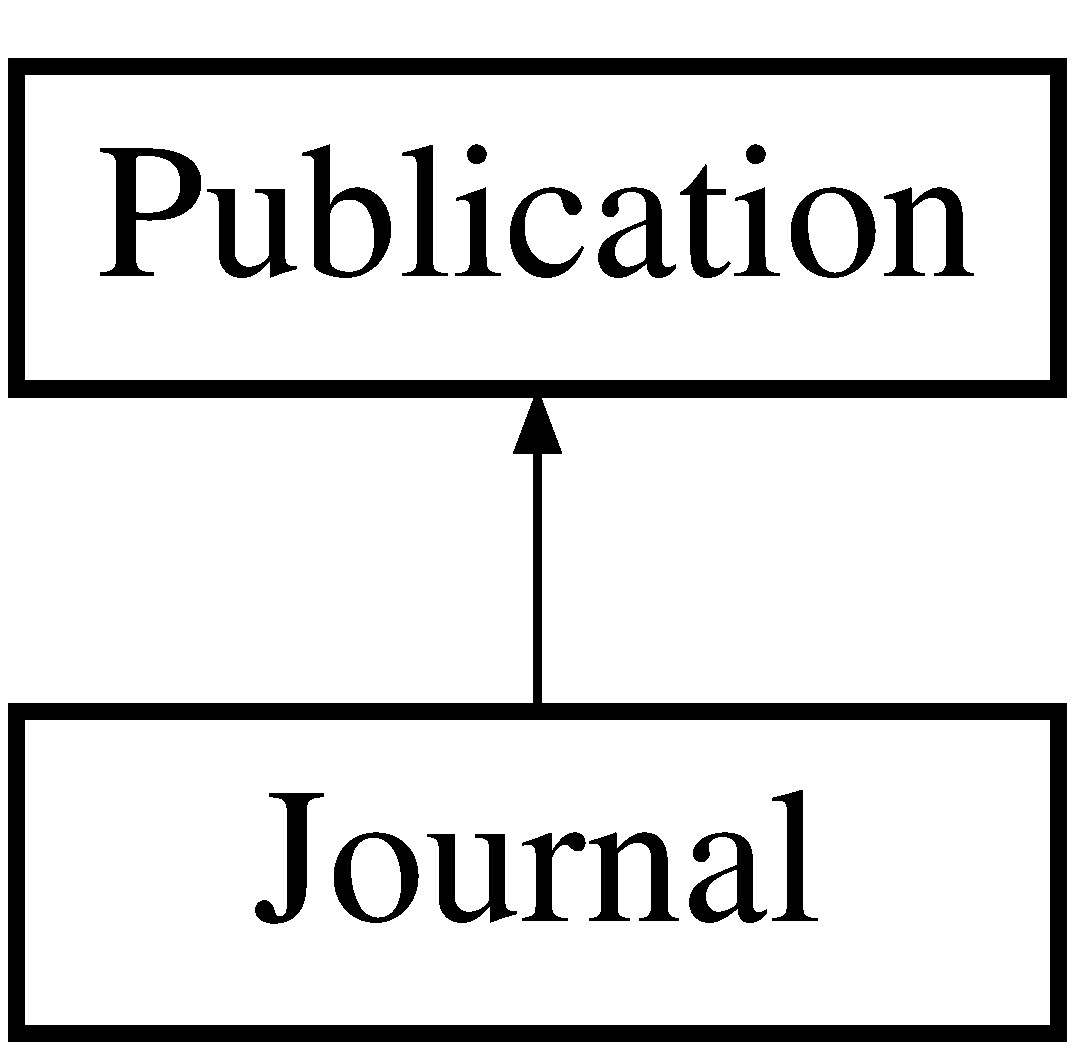
\includegraphics[height=2.000000cm]{class_journal}
\end{center}
\end{figure}
\subsection*{Public Member Functions}
\begin{DoxyCompactItemize}
\item 
\hyperlink{class_journal_aece55c5ddbc4e548d7183731a527dca3}{Journal} (int id, std\+::string desc, std\+::string col, int vol, int n, int y)
\begin{DoxyCompactList}\small\item\em \hyperlink{class_journal}{Journal} Default constructor. \end{DoxyCompactList}\item 
void \hyperlink{class_journal_a7131809f3865fbdcbba5f38996d29c7a}{show} ()
\begin{DoxyCompactList}\small\item\em Displays the information of the journal (his parameters) \end{DoxyCompactList}\item 
int \hyperlink{class_journal_af853578ebebf1297419889c2f1b5cfc9}{get\+Volume} () const
\begin{DoxyCompactList}\small\item\em Gets the volume of the journal. \end{DoxyCompactList}\item 
int \hyperlink{class_journal_ae2ee9253549e4748814119dd8ad01d2c}{get\+Number} () const
\begin{DoxyCompactList}\small\item\em Gets the number of the journal. \end{DoxyCompactList}\item 
int \hyperlink{class_journal_a9db201ef096712da288a3f3df0d86125}{get\+Year} () const
\begin{DoxyCompactList}\small\item\em Gets the year of the journal. \end{DoxyCompactList}\item 
std\+::string \hyperlink{class_journal_a631e4fa39c9875db342ed8eb1a9f5eb6}{get\+Out\+Put} (int type)
\begin{DoxyCompactList}\small\item\em Gets the output to right in the file. \end{DoxyCompactList}\item 
int \hyperlink{class_journal_ad787716ffbd1d22623245cf98c13ac4a}{get\+Type} () const
\begin{DoxyCompactList}\small\item\em Gets the type of the \hyperlink{class_journal}{Journal}. \end{DoxyCompactList}\end{DoxyCompactItemize}
\subsection*{Additional Inherited Members}


\subsection{Detailed Description}
Class \hyperlink{class_journal}{Journal} -\/ creates the object \hyperlink{class_journal}{Journal} -\/ type of \hyperlink{class_publication}{Publication}. 

\subsection{Constructor \& Destructor Documentation}
\mbox{\Hypertarget{class_journal_aece55c5ddbc4e548d7183731a527dca3}\label{class_journal_aece55c5ddbc4e548d7183731a527dca3}} 
\index{Journal@{Journal}!Journal@{Journal}}
\index{Journal@{Journal}!Journal@{Journal}}
\subsubsection{\texorpdfstring{Journal()}{Journal()}}
{\footnotesize\ttfamily Journal\+::\+Journal (\begin{DoxyParamCaption}\item[{int}]{id,  }\item[{std\+::string}]{desc,  }\item[{std\+::string}]{col,  }\item[{int}]{vol,  }\item[{int}]{n,  }\item[{int}]{y }\end{DoxyParamCaption})}



\hyperlink{class_journal}{Journal} Default constructor. 


\begin{DoxyParams}{Parameters}
{\em id} & unique way to identify all the journals \\
\hline
{\em desc} & description of the journal \\
\hline
{\em col} & collecting of the journal \\
\hline
{\em vol} & volume \\
\hline
{\em n} & number \\
\hline
{\em y} & year when the journal was published \\
\hline
\end{DoxyParams}


\subsection{Member Function Documentation}
\mbox{\Hypertarget{class_journal_ae2ee9253549e4748814119dd8ad01d2c}\label{class_journal_ae2ee9253549e4748814119dd8ad01d2c}} 
\index{Journal@{Journal}!get\+Number@{get\+Number}}
\index{get\+Number@{get\+Number}!Journal@{Journal}}
\subsubsection{\texorpdfstring{get\+Number()}{getNumber()}}
{\footnotesize\ttfamily int Journal\+::get\+Number (\begin{DoxyParamCaption}{ }\end{DoxyParamCaption}) const}



Gets the number of the journal. 

\begin{DoxyReturn}{Returns}
Respective number 
\end{DoxyReturn}
\mbox{\Hypertarget{class_journal_a631e4fa39c9875db342ed8eb1a9f5eb6}\label{class_journal_a631e4fa39c9875db342ed8eb1a9f5eb6}} 
\index{Journal@{Journal}!get\+Out\+Put@{get\+Out\+Put}}
\index{get\+Out\+Put@{get\+Out\+Put}!Journal@{Journal}}
\subsubsection{\texorpdfstring{get\+Out\+Put()}{getOutPut()}}
{\footnotesize\ttfamily string Journal\+::get\+Out\+Put (\begin{DoxyParamCaption}\item[{int}]{type }\end{DoxyParamCaption})\hspace{0.3cm}{\ttfamily [virtual]}}



Gets the output to right in the file. 


\begin{DoxyParams}{Parameters}
{\em type} & integer type of the publication, 0 if \hyperlink{class_book}{Book} and 1 if \hyperlink{class_journal}{Journal}\\
\hline
\end{DoxyParams}
\begin{DoxyReturn}{Returns}
the string to be written into the file 
\end{DoxyReturn}


Reimplemented from \hyperlink{class_publication_af382f9557807e8375478ceb7890e841f}{Publication}.

\mbox{\Hypertarget{class_journal_ad787716ffbd1d22623245cf98c13ac4a}\label{class_journal_ad787716ffbd1d22623245cf98c13ac4a}} 
\index{Journal@{Journal}!get\+Type@{get\+Type}}
\index{get\+Type@{get\+Type}!Journal@{Journal}}
\subsubsection{\texorpdfstring{get\+Type()}{getType()}}
{\footnotesize\ttfamily int Journal\+::get\+Type (\begin{DoxyParamCaption}{ }\end{DoxyParamCaption}) const\hspace{0.3cm}{\ttfamily [virtual]}}



Gets the type of the \hyperlink{class_journal}{Journal}. 

\begin{DoxyReturn}{Returns}
type of the \hyperlink{class_publication}{Publication} (\hyperlink{class_book}{Book} or \hyperlink{class_journal}{Journal}) 
\end{DoxyReturn}


Reimplemented from \hyperlink{class_publication_ab0bd9119b29b09fbbe9044016a512407}{Publication}.

\mbox{\Hypertarget{class_journal_af853578ebebf1297419889c2f1b5cfc9}\label{class_journal_af853578ebebf1297419889c2f1b5cfc9}} 
\index{Journal@{Journal}!get\+Volume@{get\+Volume}}
\index{get\+Volume@{get\+Volume}!Journal@{Journal}}
\subsubsection{\texorpdfstring{get\+Volume()}{getVolume()}}
{\footnotesize\ttfamily int Journal\+::get\+Volume (\begin{DoxyParamCaption}{ }\end{DoxyParamCaption}) const}



Gets the volume of the journal. 

\begin{DoxyReturn}{Returns}
Respective volume 
\end{DoxyReturn}
\mbox{\Hypertarget{class_journal_a9db201ef096712da288a3f3df0d86125}\label{class_journal_a9db201ef096712da288a3f3df0d86125}} 
\index{Journal@{Journal}!get\+Year@{get\+Year}}
\index{get\+Year@{get\+Year}!Journal@{Journal}}
\subsubsection{\texorpdfstring{get\+Year()}{getYear()}}
{\footnotesize\ttfamily int Journal\+::get\+Year (\begin{DoxyParamCaption}{ }\end{DoxyParamCaption}) const}



Gets the year of the journal. 

\begin{DoxyReturn}{Returns}
Respective year 
\end{DoxyReturn}
\mbox{\Hypertarget{class_journal_a7131809f3865fbdcbba5f38996d29c7a}\label{class_journal_a7131809f3865fbdcbba5f38996d29c7a}} 
\index{Journal@{Journal}!show@{show}}
\index{show@{show}!Journal@{Journal}}
\subsubsection{\texorpdfstring{show()}{show()}}
{\footnotesize\ttfamily void Journal\+::show (\begin{DoxyParamCaption}{ }\end{DoxyParamCaption})\hspace{0.3cm}{\ttfamily [virtual]}}



Displays the information of the journal (his parameters) 

\begin{DoxyReturn}{Returns}
void 
\end{DoxyReturn}


Reimplemented from \hyperlink{class_publication_aa4240a04fcecd6257e0d1a33e8f18ff0}{Publication}.



The documentation for this class was generated from the following files\+:\begin{DoxyCompactItemize}
\item 
Journal.\+h\item 
Journal.\+cpp\end{DoxyCompactItemize}

\hypertarget{class_production___request}{}\section{Production\+\_\+\+Request Class Reference}
\label{class_production___request}\index{Production\+\_\+\+Request@{Production\+\_\+\+Request}}


Class Production request to be done by \hyperlink{class_headquarters}{Headquarters}.  




{\ttfamily \#include $<$Production\+\_\+\+Request.\+h$>$}

\subsection*{Public Member Functions}
\begin{DoxyCompactItemize}
\item 
\hyperlink{class_production___request_a0c2c84b7434099e897226a93713dd050}{Production\+\_\+\+Request} (int id, int p\+\_\+id, \hyperlink{class_date}{Date} d1, \hyperlink{class_date}{Date} d2, int q)
\begin{DoxyCompactList}\small\item\em default constructor of the object \end{DoxyCompactList}\item 
void \hyperlink{class_production___request_ab08bac86aa95f28f06bf17685f7164aa}{show} ()
\begin{DoxyCompactList}\small\item\em displays the information of the production request (his parameters) \end{DoxyCompactList}\item 
int \hyperlink{class_production___request_ae2448a51f3bdab909bdc53f2e5bae666}{get\+ID} () const
\begin{DoxyCompactList}\small\item\em gets the ID of the production request \end{DoxyCompactList}\item 
int \hyperlink{class_production___request_aafa7c4bbaae9dc72c8954a6e1eaff817}{get\+Publication\+ID} () const
\begin{DoxyCompactList}\small\item\em the publication ID of the publication request \end{DoxyCompactList}\item 
\hyperlink{class_date}{Date} \hyperlink{class_production___request_aed0efd10e677d4bca14d00b5f981718a}{get\+Request\+Date} () const
\begin{DoxyCompactList}\small\item\em gets the request date of the publication order \end{DoxyCompactList}\item 
\hyperlink{class_date}{Date} \hyperlink{class_production___request_a3df39092c2aac5a34401f38a29097b3a}{get\+Deadline} () const
\begin{DoxyCompactList}\small\item\em gets the deadline of the publication request \end{DoxyCompactList}\item 
int \hyperlink{class_production___request_aac38238db2c32af73c839314c3e254a6}{get\+Quantity} () const
\begin{DoxyCompactList}\small\item\em gets the quantity of the publication order \end{DoxyCompactList}\item 
bool \hyperlink{class_production___request_a37fd21082c7c874be9587e8d3cce7174}{operator==} (\hyperlink{class_production___request}{Production\+\_\+\+Request} \&pr2) const
\begin{DoxyCompactList}\small\item\em operator == for the \hyperlink{class_production___request}{Production\+\_\+\+Request} \end{DoxyCompactList}\item 
bool \hyperlink{class_production___request_acf3db397822496809bde807696518e95}{operator$<$} (const \hyperlink{class_production___request}{Production\+\_\+\+Request} \&pr2) const
\begin{DoxyCompactList}\small\item\em operator $<$ for the \hyperlink{class_production___request}{Production\+\_\+\+Request} \end{DoxyCompactList}\item 
void \hyperlink{class_production___request_a3329479425a0e91eec8cf2f8fabc185e}{set\+\_\+\+Deadline} (int year, int month, int day)
\begin{DoxyCompactList}\small\item\em Changes the Deadline of the \hyperlink{class_production___request}{Production\+\_\+\+Request}. \end{DoxyCompactList}\end{DoxyCompactItemize}


\subsection{Detailed Description}
Class Production request to be done by \hyperlink{class_headquarters}{Headquarters}. 

\subsection{Constructor \& Destructor Documentation}
\mbox{\Hypertarget{class_production___request_a0c2c84b7434099e897226a93713dd050}\label{class_production___request_a0c2c84b7434099e897226a93713dd050}} 
\index{Production\+\_\+\+Request@{Production\+\_\+\+Request}!Production\+\_\+\+Request@{Production\+\_\+\+Request}}
\index{Production\+\_\+\+Request@{Production\+\_\+\+Request}!Production\+\_\+\+Request@{Production\+\_\+\+Request}}
\subsubsection{\texorpdfstring{Production\+\_\+\+Request()}{Production\_Request()}}
{\footnotesize\ttfamily Production\+\_\+\+Request\+::\+Production\+\_\+\+Request (\begin{DoxyParamCaption}\item[{int}]{id,  }\item[{int}]{p\+\_\+id,  }\item[{\hyperlink{class_date}{Date}}]{d1,  }\item[{\hyperlink{class_date}{Date}}]{d2,  }\item[{int}]{q }\end{DoxyParamCaption})}



default constructor of the object 


\begin{DoxyParams}{Parameters}
{\em id} & is the unique way to identify the production request \\
\hline
{\em p\+\_\+id} & is the id of the publication (book or journal) \\
\hline
{\em d1} & is the request date of the order \\
\hline
{\em d2} & is the deadline of the request \\
\hline
{\em q} & is the quantity of the request, publication (book or journal) \\
\hline
\end{DoxyParams}


\subsection{Member Function Documentation}
\mbox{\Hypertarget{class_production___request_a3df39092c2aac5a34401f38a29097b3a}\label{class_production___request_a3df39092c2aac5a34401f38a29097b3a}} 
\index{Production\+\_\+\+Request@{Production\+\_\+\+Request}!get\+Deadline@{get\+Deadline}}
\index{get\+Deadline@{get\+Deadline}!Production\+\_\+\+Request@{Production\+\_\+\+Request}}
\subsubsection{\texorpdfstring{get\+Deadline()}{getDeadline()}}
{\footnotesize\ttfamily \hyperlink{class_date}{Date} Production\+\_\+\+Request\+::get\+Deadline (\begin{DoxyParamCaption}{ }\end{DoxyParamCaption}) const}



gets the deadline of the publication request 

\begin{DoxyReturn}{Returns}
the delivery date 
\end{DoxyReturn}
\mbox{\Hypertarget{class_production___request_ae2448a51f3bdab909bdc53f2e5bae666}\label{class_production___request_ae2448a51f3bdab909bdc53f2e5bae666}} 
\index{Production\+\_\+\+Request@{Production\+\_\+\+Request}!get\+ID@{get\+ID}}
\index{get\+ID@{get\+ID}!Production\+\_\+\+Request@{Production\+\_\+\+Request}}
\subsubsection{\texorpdfstring{get\+I\+D()}{getID()}}
{\footnotesize\ttfamily int Production\+\_\+\+Request\+::get\+ID (\begin{DoxyParamCaption}{ }\end{DoxyParamCaption}) const}



gets the ID of the production request 

\begin{DoxyReturn}{Returns}
the respective ID 
\end{DoxyReturn}
\mbox{\Hypertarget{class_production___request_aafa7c4bbaae9dc72c8954a6e1eaff817}\label{class_production___request_aafa7c4bbaae9dc72c8954a6e1eaff817}} 
\index{Production\+\_\+\+Request@{Production\+\_\+\+Request}!get\+Publication\+ID@{get\+Publication\+ID}}
\index{get\+Publication\+ID@{get\+Publication\+ID}!Production\+\_\+\+Request@{Production\+\_\+\+Request}}
\subsubsection{\texorpdfstring{get\+Publication\+I\+D()}{getPublicationID()}}
{\footnotesize\ttfamily int Production\+\_\+\+Request\+::get\+Publication\+ID (\begin{DoxyParamCaption}{ }\end{DoxyParamCaption}) const}



the publication ID of the publication request 

\begin{DoxyReturn}{Returns}
the respective publication ID 
\end{DoxyReturn}
\mbox{\Hypertarget{class_production___request_aac38238db2c32af73c839314c3e254a6}\label{class_production___request_aac38238db2c32af73c839314c3e254a6}} 
\index{Production\+\_\+\+Request@{Production\+\_\+\+Request}!get\+Quantity@{get\+Quantity}}
\index{get\+Quantity@{get\+Quantity}!Production\+\_\+\+Request@{Production\+\_\+\+Request}}
\subsubsection{\texorpdfstring{get\+Quantity()}{getQuantity()}}
{\footnotesize\ttfamily int Production\+\_\+\+Request\+::get\+Quantity (\begin{DoxyParamCaption}{ }\end{DoxyParamCaption}) const}



gets the quantity of the publication order 

\begin{DoxyReturn}{Returns}
the respective quantity 
\end{DoxyReturn}
\mbox{\Hypertarget{class_production___request_aed0efd10e677d4bca14d00b5f981718a}\label{class_production___request_aed0efd10e677d4bca14d00b5f981718a}} 
\index{Production\+\_\+\+Request@{Production\+\_\+\+Request}!get\+Request\+Date@{get\+Request\+Date}}
\index{get\+Request\+Date@{get\+Request\+Date}!Production\+\_\+\+Request@{Production\+\_\+\+Request}}
\subsubsection{\texorpdfstring{get\+Request\+Date()}{getRequestDate()}}
{\footnotesize\ttfamily \hyperlink{class_date}{Date} Production\+\_\+\+Request\+::get\+Request\+Date (\begin{DoxyParamCaption}{ }\end{DoxyParamCaption}) const}



gets the request date of the publication order 

\begin{DoxyReturn}{Returns}
the request date 
\end{DoxyReturn}
\mbox{\Hypertarget{class_production___request_acf3db397822496809bde807696518e95}\label{class_production___request_acf3db397822496809bde807696518e95}} 
\index{Production\+\_\+\+Request@{Production\+\_\+\+Request}!operator$<$@{operator$<$}}
\index{operator$<$@{operator$<$}!Production\+\_\+\+Request@{Production\+\_\+\+Request}}
\subsubsection{\texorpdfstring{operator$<$()}{operator<()}}
{\footnotesize\ttfamily bool Production\+\_\+\+Request\+::operator$<$ (\begin{DoxyParamCaption}\item[{const \hyperlink{class_production___request}{Production\+\_\+\+Request} \&}]{pr2 }\end{DoxyParamCaption}) const}



operator $<$ for the \hyperlink{class_production___request}{Production\+\_\+\+Request} 


\begin{DoxyParams}{Parameters}
{\em the} & \hyperlink{class_production___request}{Production\+\_\+\+Request} pr2 to the compared\\
\hline
\end{DoxyParams}
\begin{DoxyReturn}{Returns}
true if the Production\+\_\+\+Requests is less than pr2 and false otherwise 
\end{DoxyReturn}
\mbox{\Hypertarget{class_production___request_a37fd21082c7c874be9587e8d3cce7174}\label{class_production___request_a37fd21082c7c874be9587e8d3cce7174}} 
\index{Production\+\_\+\+Request@{Production\+\_\+\+Request}!operator==@{operator==}}
\index{operator==@{operator==}!Production\+\_\+\+Request@{Production\+\_\+\+Request}}
\subsubsection{\texorpdfstring{operator==()}{operator==()}}
{\footnotesize\ttfamily bool Production\+\_\+\+Request\+::operator== (\begin{DoxyParamCaption}\item[{\hyperlink{class_production___request}{Production\+\_\+\+Request} \&}]{pr2 }\end{DoxyParamCaption}) const}



operator == for the \hyperlink{class_production___request}{Production\+\_\+\+Request} 


\begin{DoxyParams}{Parameters}
{\em the} & \hyperlink{class_production___request}{Production\+\_\+\+Request} pr2 to the compared\\
\hline
\end{DoxyParams}
\begin{DoxyReturn}{Returns}
true if the Production\+\_\+\+Requests are equal and false otherwise 
\end{DoxyReturn}
\mbox{\Hypertarget{class_production___request_a3329479425a0e91eec8cf2f8fabc185e}\label{class_production___request_a3329479425a0e91eec8cf2f8fabc185e}} 
\index{Production\+\_\+\+Request@{Production\+\_\+\+Request}!set\+\_\+\+Deadline@{set\+\_\+\+Deadline}}
\index{set\+\_\+\+Deadline@{set\+\_\+\+Deadline}!Production\+\_\+\+Request@{Production\+\_\+\+Request}}
\subsubsection{\texorpdfstring{set\+\_\+\+Deadline()}{set\_Deadline()}}
{\footnotesize\ttfamily void Production\+\_\+\+Request\+::set\+\_\+\+Deadline (\begin{DoxyParamCaption}\item[{int}]{year,  }\item[{int}]{month,  }\item[{int}]{day }\end{DoxyParamCaption})}



Changes the Deadline of the \hyperlink{class_production___request}{Production\+\_\+\+Request}. 


\begin{DoxyParams}{Parameters}
{\em year} & year of the new Deadline\\
\hline
{\em month} & month of the new Deadline\\
\hline
{\em day} & day of the new Deadline\\
\hline
\end{DoxyParams}
\begin{DoxyReturn}{Returns}
void 
\end{DoxyReturn}
\mbox{\Hypertarget{class_production___request_ab08bac86aa95f28f06bf17685f7164aa}\label{class_production___request_ab08bac86aa95f28f06bf17685f7164aa}} 
\index{Production\+\_\+\+Request@{Production\+\_\+\+Request}!show@{show}}
\index{show@{show}!Production\+\_\+\+Request@{Production\+\_\+\+Request}}
\subsubsection{\texorpdfstring{show()}{show()}}
{\footnotesize\ttfamily void Production\+\_\+\+Request\+::show (\begin{DoxyParamCaption}{ }\end{DoxyParamCaption})}



displays the information of the production request (his parameters) 

\begin{DoxyReturn}{Returns}
void 
\end{DoxyReturn}


The documentation for this class was generated from the following files\+:\begin{DoxyCompactItemize}
\item 
D\+:/\+F\+E\+U\+P/\+M\+I\+E\+I\+C/2º ano/\+A\+E\+D\+A/\+Projeto\+\_\+\+Eclipse/as/src/Production\+\_\+\+Request.\+h\item 
D\+:/\+F\+E\+U\+P/\+M\+I\+E\+I\+C/2º ano/\+A\+E\+D\+A/\+Projeto\+\_\+\+Eclipse/as/src/Production\+\_\+\+Request.\+cpp\end{DoxyCompactItemize}

\hypertarget{class_publication}{}\section{Publication Class Reference}
\label{class_publication}\index{Publication@{Publication}}


Class \hyperlink{class_publication}{Publication}, abstract, Class parent of \hyperlink{class_book}{Book} and \hyperlink{class_journal}{Journal}.  




{\ttfamily \#include $<$Publication.\+h$>$}

Inheritance diagram for Publication\+:\begin{figure}[H]
\begin{center}
\leavevmode
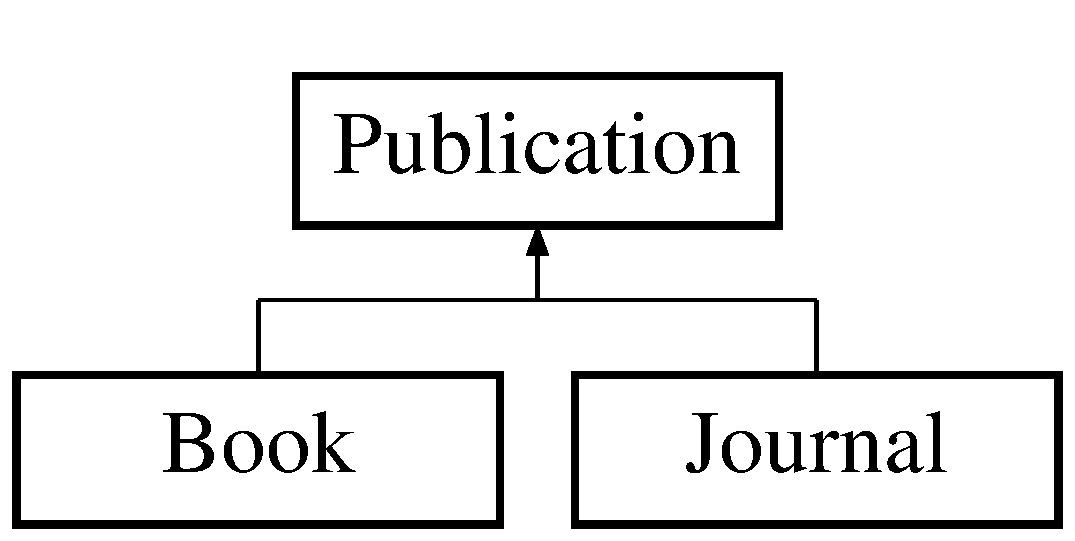
\includegraphics[height=2.000000cm]{class_publication}
\end{center}
\end{figure}
\subsection*{Public Member Functions}
\begin{DoxyCompactItemize}
\item 
\hyperlink{class_publication_ab271fddf4b63d13af271f47979e9c4a7}{Publication} (int id, std\+::string desc, std\+::string col)
\begin{DoxyCompactList}\small\item\em Default constructor of the publication. \end{DoxyCompactList}\item 
virtual void \hyperlink{class_publication_aa4240a04fcecd6257e0d1a33e8f18ff0}{show} ()
\begin{DoxyCompactList}\small\item\em Displays the information of the \hyperlink{class_publication}{Publication}. \end{DoxyCompactList}\item 
int \hyperlink{class_publication_ab1b5251a7e94efcb7792edbac4ff93bc}{get\+ID} () const
\begin{DoxyCompactList}\small\item\em Gets the ID of \hyperlink{class_publication}{Publication}. \end{DoxyCompactList}\item 
std\+::string \hyperlink{class_publication_a5cc83441c3e2dd8daaa050a18b2e6bdd}{get\+Descripiton} () const
\begin{DoxyCompactList}\small\item\em Gets the description of the \hyperlink{class_publication}{Publication}. \end{DoxyCompactList}\item 
std\+::string \hyperlink{class_publication_ae1005ffcb387e2c1cd79483fdbb545c8}{get\+Colection} () const
\begin{DoxyCompactList}\small\item\em Gets the collection of the \hyperlink{class_publication}{Publication}. \end{DoxyCompactList}\item 
bool \hyperlink{class_publication_a60f079ac47aa4b8aa94957e15f12a2da}{operator==} (const \hyperlink{class_publication}{Publication} \&p2) const
\begin{DoxyCompactList}\small\item\em operator == for the publication \end{DoxyCompactList}\item 
virtual int \hyperlink{class_publication_ab0bd9119b29b09fbbe9044016a512407}{get\+Type} () const
\begin{DoxyCompactList}\small\item\em Get the type of the publication 0 if \hyperlink{class_book}{Book} or 1 if \hyperlink{class_journal}{Journal}. \end{DoxyCompactList}\item 
virtual std\+::string \hyperlink{class_publication_af382f9557807e8375478ceb7890e841f}{get\+Out\+Put} (int type)
\begin{DoxyCompactList}\small\item\em Gets the output to right in the file. \end{DoxyCompactList}\end{DoxyCompactItemize}
\subsection*{Protected Attributes}
\begin{DoxyCompactItemize}
\item 
\mbox{\Hypertarget{class_publication_a5bb18d963c10a67fcc6da7b895a3474a}\label{class_publication_a5bb18d963c10a67fcc6da7b895a3474a}} 
int \hyperlink{class_publication_a5bb18d963c10a67fcc6da7b895a3474a}{ID}
\begin{DoxyCompactList}\small\item\em ID of the publication (book or journal) \end{DoxyCompactList}\item 
\mbox{\Hypertarget{class_publication_abfcf695658989bad9371a7896213f9a6}\label{class_publication_abfcf695658989bad9371a7896213f9a6}} 
std\+::string \hyperlink{class_publication_abfcf695658989bad9371a7896213f9a6}{description}
\begin{DoxyCompactList}\small\item\em description of the publication \end{DoxyCompactList}\item 
\mbox{\Hypertarget{class_publication_a644dc37a95f7da3bc8b83ca601383368}\label{class_publication_a644dc37a95f7da3bc8b83ca601383368}} 
std\+::string \hyperlink{class_publication_a644dc37a95f7da3bc8b83ca601383368}{colection}
\begin{DoxyCompactList}\small\item\em collection of the publication \end{DoxyCompactList}\end{DoxyCompactItemize}


\subsection{Detailed Description}
Class \hyperlink{class_publication}{Publication}, abstract, Class parent of \hyperlink{class_book}{Book} and \hyperlink{class_journal}{Journal}. 

\subsection{Constructor \& Destructor Documentation}
\mbox{\Hypertarget{class_publication_ab271fddf4b63d13af271f47979e9c4a7}\label{class_publication_ab271fddf4b63d13af271f47979e9c4a7}} 
\index{Publication@{Publication}!Publication@{Publication}}
\index{Publication@{Publication}!Publication@{Publication}}
\subsubsection{\texorpdfstring{Publication()}{Publication()}}
{\footnotesize\ttfamily Publication\+::\+Publication (\begin{DoxyParamCaption}\item[{int}]{id,  }\item[{std\+::string}]{desc,  }\item[{std\+::string}]{col }\end{DoxyParamCaption})}



Default constructor of the publication. 


\begin{DoxyParams}{Parameters}
{\em id} & unique way to identify the publication \\
\hline
{\em desc} & description of the publication \\
\hline
{\em col} & collecting of the publication \\
\hline
\end{DoxyParams}


\subsection{Member Function Documentation}
\mbox{\Hypertarget{class_publication_ae1005ffcb387e2c1cd79483fdbb545c8}\label{class_publication_ae1005ffcb387e2c1cd79483fdbb545c8}} 
\index{Publication@{Publication}!get\+Colection@{get\+Colection}}
\index{get\+Colection@{get\+Colection}!Publication@{Publication}}
\subsubsection{\texorpdfstring{get\+Colection()}{getColection()}}
{\footnotesize\ttfamily string Publication\+::get\+Colection (\begin{DoxyParamCaption}{ }\end{DoxyParamCaption}) const}



Gets the collection of the \hyperlink{class_publication}{Publication}. 

\begin{DoxyReturn}{Returns}
Collection of the \hyperlink{class_publication}{Publication} in a string 
\end{DoxyReturn}
\mbox{\Hypertarget{class_publication_a5cc83441c3e2dd8daaa050a18b2e6bdd}\label{class_publication_a5cc83441c3e2dd8daaa050a18b2e6bdd}} 
\index{Publication@{Publication}!get\+Descripiton@{get\+Descripiton}}
\index{get\+Descripiton@{get\+Descripiton}!Publication@{Publication}}
\subsubsection{\texorpdfstring{get\+Descripiton()}{getDescripiton()}}
{\footnotesize\ttfamily string Publication\+::get\+Descripiton (\begin{DoxyParamCaption}{ }\end{DoxyParamCaption}) const}



Gets the description of the \hyperlink{class_publication}{Publication}. 

\begin{DoxyReturn}{Returns}
Description of the \hyperlink{class_publication}{Publication} in a string 
\end{DoxyReturn}
\mbox{\Hypertarget{class_publication_ab1b5251a7e94efcb7792edbac4ff93bc}\label{class_publication_ab1b5251a7e94efcb7792edbac4ff93bc}} 
\index{Publication@{Publication}!get\+ID@{get\+ID}}
\index{get\+ID@{get\+ID}!Publication@{Publication}}
\subsubsection{\texorpdfstring{get\+I\+D()}{getID()}}
{\footnotesize\ttfamily int Publication\+::get\+ID (\begin{DoxyParamCaption}{ }\end{DoxyParamCaption}) const}



Gets the ID of \hyperlink{class_publication}{Publication}. 

\begin{DoxyReturn}{Returns}
Respective ID 
\end{DoxyReturn}
\mbox{\Hypertarget{class_publication_af382f9557807e8375478ceb7890e841f}\label{class_publication_af382f9557807e8375478ceb7890e841f}} 
\index{Publication@{Publication}!get\+Out\+Put@{get\+Out\+Put}}
\index{get\+Out\+Put@{get\+Out\+Put}!Publication@{Publication}}
\subsubsection{\texorpdfstring{get\+Out\+Put()}{getOutPut()}}
{\footnotesize\ttfamily string Publication\+::get\+Out\+Put (\begin{DoxyParamCaption}\item[{int}]{type }\end{DoxyParamCaption})\hspace{0.3cm}{\ttfamily [virtual]}}



Gets the output to right in the file. 


\begin{DoxyParams}{Parameters}
{\em type} & is the integer type of the publication, 0 if \hyperlink{class_book}{Book} and 1 if \hyperlink{class_journal}{Journal}\\
\hline
\end{DoxyParams}
\begin{DoxyReturn}{Returns}
string to write to the file 
\end{DoxyReturn}


Reimplemented in \hyperlink{class_journal_a631e4fa39c9875db342ed8eb1a9f5eb6}{Journal}, and \hyperlink{class_book_ab72570b8b4d902d6f3fe681dc29b2198}{Book}.

\mbox{\Hypertarget{class_publication_ab0bd9119b29b09fbbe9044016a512407}\label{class_publication_ab0bd9119b29b09fbbe9044016a512407}} 
\index{Publication@{Publication}!get\+Type@{get\+Type}}
\index{get\+Type@{get\+Type}!Publication@{Publication}}
\subsubsection{\texorpdfstring{get\+Type()}{getType()}}
{\footnotesize\ttfamily virtual int Publication\+::get\+Type (\begin{DoxyParamCaption}{ }\end{DoxyParamCaption}) const\hspace{0.3cm}{\ttfamily [inline]}, {\ttfamily [virtual]}}



Get the type of the publication 0 if \hyperlink{class_book}{Book} or 1 if \hyperlink{class_journal}{Journal}. 

\begin{DoxyReturn}{Returns}
type (integer) 
\end{DoxyReturn}


Reimplemented in \hyperlink{class_journal_ad787716ffbd1d22623245cf98c13ac4a}{Journal}, and \hyperlink{class_book_a285dd3654bfced6baffd86320c39d42e}{Book}.

\mbox{\Hypertarget{class_publication_a60f079ac47aa4b8aa94957e15f12a2da}\label{class_publication_a60f079ac47aa4b8aa94957e15f12a2da}} 
\index{Publication@{Publication}!operator==@{operator==}}
\index{operator==@{operator==}!Publication@{Publication}}
\subsubsection{\texorpdfstring{operator==()}{operator==()}}
{\footnotesize\ttfamily bool Publication\+::operator== (\begin{DoxyParamCaption}\item[{const \hyperlink{class_publication}{Publication} \&}]{p2 }\end{DoxyParamCaption}) const}



operator == for the publication 


\begin{DoxyParams}{Parameters}
{\em the} & \hyperlink{class_publication}{Publication} p2 to the compared\\
\hline
\end{DoxyParams}
\begin{DoxyReturn}{Returns}
true if the Publications are equal and false otherwise 
\end{DoxyReturn}
\mbox{\Hypertarget{class_publication_aa4240a04fcecd6257e0d1a33e8f18ff0}\label{class_publication_aa4240a04fcecd6257e0d1a33e8f18ff0}} 
\index{Publication@{Publication}!show@{show}}
\index{show@{show}!Publication@{Publication}}
\subsubsection{\texorpdfstring{show()}{show()}}
{\footnotesize\ttfamily void Publication\+::show (\begin{DoxyParamCaption}{ }\end{DoxyParamCaption})\hspace{0.3cm}{\ttfamily [virtual]}}



Displays the information of the \hyperlink{class_publication}{Publication}. 

because publications is an abstract class and the \hyperlink{class_publication_aa4240a04fcecd6257e0d1a33e8f18ff0}{show()} function is initialized in book and journal classes

\begin{DoxyReturn}{Returns}
void 
\end{DoxyReturn}


Reimplemented in \hyperlink{class_journal_a7131809f3865fbdcbba5f38996d29c7a}{Journal}, and \hyperlink{class_book_a8368f243d8a645444e8019760a50cc8b}{Book}.



The documentation for this class was generated from the following files\+:\begin{DoxyCompactItemize}
\item 
Publication.\+h\item 
Publication.\+cpp\end{DoxyCompactItemize}

\hypertarget{class_store}{}\section{Store Class Reference}
\label{class_store}\index{Store@{Store}}


Class \hyperlink{class_store}{Store} -\/ creates an object \hyperlink{class_store}{Store}.  




{\ttfamily \#include $<$Store.\+h$>$}

\subsection*{Public Member Functions}
\begin{DoxyCompactItemize}
\item 
\hyperlink{class_store_a7e67d8e31c81dd0ae4a8fa5a397a40df}{Store} (int id, std\+::string city, unsigned long pn)
\begin{DoxyCompactList}\small\item\em Default constructor. \end{DoxyCompactList}\item 
void \hyperlink{class_store_a7c3951daba9c6f0c3c432aea46cfd5b8}{show} ()
\begin{DoxyCompactList}\small\item\em Displays the information of the \hyperlink{class_store}{Store} (his parameters) \end{DoxyCompactList}\item 
int \hyperlink{class_store_aaaf0609bbd37babf36a4b9afb09709cf}{get\+ID} () const
\begin{DoxyCompactList}\small\item\em Gets the ID of the \hyperlink{class_store}{Store}. \end{DoxyCompactList}\item 
std\+::string \hyperlink{class_store_a63032ec1afe4b301f55584a8018f478c}{get\+City} () const
\begin{DoxyCompactList}\small\item\em Gets the City of the \hyperlink{class_store}{Store}. \end{DoxyCompactList}\item 
\hyperlink{class_employee}{Employee} \hyperlink{class_store_ab4b4d6e958e7d26398f3e6e0e932c920}{get\+Worker} () const
\begin{DoxyCompactList}\small\item\em Gets the \hyperlink{class_employee}{Employee} of the \hyperlink{class_store}{Store}. \end{DoxyCompactList}\item 
unsigned long \hyperlink{class_store_afbef10a37143ea91b200d50e8e6b83d7}{get\+Phone\+Number} () const
\begin{DoxyCompactList}\small\item\em Gets the phone number of the store. \end{DoxyCompactList}\item 
void \hyperlink{class_store_a5486a87318c219a4cc85438c9b171ffc}{set\+Worker} (\hyperlink{class_employee}{Employee} $\ast$worker)
\begin{DoxyCompactList}\small\item\em Sets the worker of the \hyperlink{class_store}{Store}. \end{DoxyCompactList}\item 
int \hyperlink{class_store_a6b828ab56ffdcf4c8eb64e53ab998543}{get\+I\+D\+\_\+employee} () const
\begin{DoxyCompactList}\small\item\em Gets the \hyperlink{class_employee}{Employee} ID. \end{DoxyCompactList}\item 
std\+::vector$<$ \hyperlink{class_publication}{Publication} $\ast$$>$ \hyperlink{class_store_a05e802d26ede5fc4225074d1c732b3f3}{get\+\_\+publications\+\_\+store} ()
\begin{DoxyCompactList}\small\item\em Gets the vector of publications (books and journals) \end{DoxyCompactList}\item 
void \hyperlink{class_store_a2d721f632d90947fae8c9eaa9f8abfcb}{set\+I\+D\+\_\+employee} (int val)
\begin{DoxyCompactList}\small\item\em Sets the \hyperlink{class_employee}{Employee} ID. \end{DoxyCompactList}\item 
void \hyperlink{class_store_aaea321fd77af274c34e8ade71ed02aa7}{add\+Publication} (\hyperlink{class_publication}{Publication} $\ast$publication, int stock\+\_\+min)
\begin{DoxyCompactList}\small\item\em Add a \hyperlink{class_publication}{Publication} (\hyperlink{class_book}{Book} or \hyperlink{class_journal}{Journal}) to the \hyperlink{class_store}{Store}. \end{DoxyCompactList}\item 
void \hyperlink{class_store_a67bad0d70942ce8560926110297fdf33}{add\+Stock} (int publication\+\_\+id, int amount)
\begin{DoxyCompactList}\small\item\em Add stock to the \hyperlink{class_publication}{Publication} (\hyperlink{class_book}{Book} or \hyperlink{class_journal}{Journal}) \end{DoxyCompactList}\item 
void \hyperlink{class_store_a64f322bc111e0e88ab0995cd86718f0d}{remove\+Publication} (int id)
\begin{DoxyCompactList}\small\item\em Removes a \hyperlink{class_publication}{Publication} of the \hyperlink{class_store}{Store}. \end{DoxyCompactList}\item 
bool \hyperlink{class_store_a4dfd27a0615f161f2f0e94297bb54969}{operator==} (\hyperlink{class_store}{Store} \&s2) const
\begin{DoxyCompactList}\small\item\em operator == for the \hyperlink{class_store}{Store} \end{DoxyCompactList}\end{DoxyCompactItemize}


\subsection{Detailed Description}
Class \hyperlink{class_store}{Store} -\/ creates an object \hyperlink{class_store}{Store}. 

\subsection{Constructor \& Destructor Documentation}
\mbox{\Hypertarget{class_store_a7e67d8e31c81dd0ae4a8fa5a397a40df}\label{class_store_a7e67d8e31c81dd0ae4a8fa5a397a40df}} 
\index{Store@{Store}!Store@{Store}}
\index{Store@{Store}!Store@{Store}}
\subsubsection{\texorpdfstring{Store()}{Store()}}
{\footnotesize\ttfamily Store\+::\+Store (\begin{DoxyParamCaption}\item[{int}]{id,  }\item[{std\+::string}]{city,  }\item[{unsigned long}]{pn }\end{DoxyParamCaption})}



Default constructor. 


\begin{DoxyParams}{Parameters}
{\em id} & unique way to identify the different stores \\
\hline
{\em city} & place where the store is situated \\
\hline
{\em pn} & phone number of the store \\
\hline
\end{DoxyParams}


\subsection{Member Function Documentation}
\mbox{\Hypertarget{class_store_aaea321fd77af274c34e8ade71ed02aa7}\label{class_store_aaea321fd77af274c34e8ade71ed02aa7}} 
\index{Store@{Store}!add\+Publication@{add\+Publication}}
\index{add\+Publication@{add\+Publication}!Store@{Store}}
\subsubsection{\texorpdfstring{add\+Publication()}{addPublication()}}
{\footnotesize\ttfamily void Store\+::add\+Publication (\begin{DoxyParamCaption}\item[{\hyperlink{class_publication}{Publication} $\ast$}]{publication,  }\item[{int}]{stock\+\_\+min }\end{DoxyParamCaption})}



Add a \hyperlink{class_publication}{Publication} (\hyperlink{class_book}{Book} or \hyperlink{class_journal}{Journal}) to the \hyperlink{class_store}{Store}. 


\begin{DoxyParams}{Parameters}
{\em publication} & book or journal to be added \\
\hline
{\em stock\+\_\+min} & minimum stock of the publication, 0 if \hyperlink{class_book}{Book} and 1 if \hyperlink{class_journal}{Journal}\\
\hline
\end{DoxyParams}
\begin{DoxyReturn}{Returns}
void 
\end{DoxyReturn}
\mbox{\Hypertarget{class_store_a67bad0d70942ce8560926110297fdf33}\label{class_store_a67bad0d70942ce8560926110297fdf33}} 
\index{Store@{Store}!add\+Stock@{add\+Stock}}
\index{add\+Stock@{add\+Stock}!Store@{Store}}
\subsubsection{\texorpdfstring{add\+Stock()}{addStock()}}
{\footnotesize\ttfamily void Store\+::add\+Stock (\begin{DoxyParamCaption}\item[{int}]{publication\+\_\+id,  }\item[{int}]{amount }\end{DoxyParamCaption})}



Add stock to the \hyperlink{class_publication}{Publication} (\hyperlink{class_book}{Book} or \hyperlink{class_journal}{Journal}) 


\begin{DoxyParams}{Parameters}
{\em publication\+\_\+id} & ID of the publication (book or journal) of the \hyperlink{class_store}{Store} to be added the respective amount \\
\hline
{\em amount} & value of the books or journals to be added on the stock of the respective publication\\
\hline
\end{DoxyParams}
\begin{DoxyReturn}{Returns}
void 
\end{DoxyReturn}
\mbox{\Hypertarget{class_store_a05e802d26ede5fc4225074d1c732b3f3}\label{class_store_a05e802d26ede5fc4225074d1c732b3f3}} 
\index{Store@{Store}!get\+\_\+publications\+\_\+store@{get\+\_\+publications\+\_\+store}}
\index{get\+\_\+publications\+\_\+store@{get\+\_\+publications\+\_\+store}!Store@{Store}}
\subsubsection{\texorpdfstring{get\+\_\+publications\+\_\+store()}{get\_publications\_store()}}
{\footnotesize\ttfamily vector$<$ \hyperlink{class_publication}{Publication} $\ast$$>$ Store\+::get\+\_\+publications\+\_\+store (\begin{DoxyParamCaption}{ }\end{DoxyParamCaption})}



Gets the vector of publications (books and journals) 

\begin{DoxyReturn}{Returns}
Respective vector 
\end{DoxyReturn}
\mbox{\Hypertarget{class_store_a63032ec1afe4b301f55584a8018f478c}\label{class_store_a63032ec1afe4b301f55584a8018f478c}} 
\index{Store@{Store}!get\+City@{get\+City}}
\index{get\+City@{get\+City}!Store@{Store}}
\subsubsection{\texorpdfstring{get\+City()}{getCity()}}
{\footnotesize\ttfamily string Store\+::get\+City (\begin{DoxyParamCaption}{ }\end{DoxyParamCaption}) const}



Gets the City of the \hyperlink{class_store}{Store}. 

\begin{DoxyReturn}{Returns}
Parameter(string) city 
\end{DoxyReturn}
\mbox{\Hypertarget{class_store_aaaf0609bbd37babf36a4b9afb09709cf}\label{class_store_aaaf0609bbd37babf36a4b9afb09709cf}} 
\index{Store@{Store}!get\+ID@{get\+ID}}
\index{get\+ID@{get\+ID}!Store@{Store}}
\subsubsection{\texorpdfstring{get\+I\+D()}{getID()}}
{\footnotesize\ttfamily int Store\+::get\+ID (\begin{DoxyParamCaption}{ }\end{DoxyParamCaption}) const}



Gets the ID of the \hyperlink{class_store}{Store}. 

\begin{DoxyReturn}{Returns}
Respective ID 
\end{DoxyReturn}
\mbox{\Hypertarget{class_store_a6b828ab56ffdcf4c8eb64e53ab998543}\label{class_store_a6b828ab56ffdcf4c8eb64e53ab998543}} 
\index{Store@{Store}!get\+I\+D\+\_\+employee@{get\+I\+D\+\_\+employee}}
\index{get\+I\+D\+\_\+employee@{get\+I\+D\+\_\+employee}!Store@{Store}}
\subsubsection{\texorpdfstring{get\+I\+D\+\_\+employee()}{getID\_employee()}}
{\footnotesize\ttfamily int Store\+::get\+I\+D\+\_\+employee (\begin{DoxyParamCaption}{ }\end{DoxyParamCaption}) const}



Gets the \hyperlink{class_employee}{Employee} ID. 

if \hyperlink{class_employee}{Employee} ID is 0, then there is no \hyperlink{class_employee}{Employee} attributed

\begin{DoxyReturn}{Returns}
Respective \hyperlink{class_employee}{Employee} ID 
\end{DoxyReturn}
\mbox{\Hypertarget{class_store_afbef10a37143ea91b200d50e8e6b83d7}\label{class_store_afbef10a37143ea91b200d50e8e6b83d7}} 
\index{Store@{Store}!get\+Phone\+Number@{get\+Phone\+Number}}
\index{get\+Phone\+Number@{get\+Phone\+Number}!Store@{Store}}
\subsubsection{\texorpdfstring{get\+Phone\+Number()}{getPhoneNumber()}}
{\footnotesize\ttfamily unsigned long Store\+::get\+Phone\+Number (\begin{DoxyParamCaption}{ }\end{DoxyParamCaption}) const}



Gets the phone number of the store. 

\begin{DoxyReturn}{Returns}
Respective phone number (parameter phone\+\_\+number) 
\end{DoxyReturn}
\mbox{\Hypertarget{class_store_ab4b4d6e958e7d26398f3e6e0e932c920}\label{class_store_ab4b4d6e958e7d26398f3e6e0e932c920}} 
\index{Store@{Store}!get\+Worker@{get\+Worker}}
\index{get\+Worker@{get\+Worker}!Store@{Store}}
\subsubsection{\texorpdfstring{get\+Worker()}{getWorker()}}
{\footnotesize\ttfamily \hyperlink{class_employee}{Employee} Store\+::get\+Worker (\begin{DoxyParamCaption}{ }\end{DoxyParamCaption}) const}



Gets the \hyperlink{class_employee}{Employee} of the \hyperlink{class_store}{Store}. 

\begin{DoxyReturn}{Returns}
\hyperlink{class_employee}{Employee} of the respective \hyperlink{class_store}{Store}, N\+U\+LL if no attributed 
\end{DoxyReturn}
\mbox{\Hypertarget{class_store_a4dfd27a0615f161f2f0e94297bb54969}\label{class_store_a4dfd27a0615f161f2f0e94297bb54969}} 
\index{Store@{Store}!operator==@{operator==}}
\index{operator==@{operator==}!Store@{Store}}
\subsubsection{\texorpdfstring{operator==()}{operator==()}}
{\footnotesize\ttfamily bool Store\+::operator== (\begin{DoxyParamCaption}\item[{\hyperlink{class_store}{Store} \&}]{s2 }\end{DoxyParamCaption}) const}



operator == for the \hyperlink{class_store}{Store} 


\begin{DoxyParams}{Parameters}
{\em s2} & \hyperlink{class_store}{Store} s2 to the compared\\
\hline
\end{DoxyParams}
\begin{DoxyReturn}{Returns}
true if the Stores are equal and false otherwise 
\end{DoxyReturn}
\mbox{\Hypertarget{class_store_a64f322bc111e0e88ab0995cd86718f0d}\label{class_store_a64f322bc111e0e88ab0995cd86718f0d}} 
\index{Store@{Store}!remove\+Publication@{remove\+Publication}}
\index{remove\+Publication@{remove\+Publication}!Store@{Store}}
\subsubsection{\texorpdfstring{remove\+Publication()}{removePublication()}}
{\footnotesize\ttfamily void Store\+::remove\+Publication (\begin{DoxyParamCaption}\item[{int}]{id }\end{DoxyParamCaption})}



Removes a \hyperlink{class_publication}{Publication} of the \hyperlink{class_store}{Store}. 


\begin{DoxyParams}{Parameters}
{\em id} & \hyperlink{class_publication}{Publication} ID that is to be removed\\
\hline
\end{DoxyParams}
\begin{DoxyReturn}{Returns}
void 
\end{DoxyReturn}
\mbox{\Hypertarget{class_store_a2d721f632d90947fae8c9eaa9f8abfcb}\label{class_store_a2d721f632d90947fae8c9eaa9f8abfcb}} 
\index{Store@{Store}!set\+I\+D\+\_\+employee@{set\+I\+D\+\_\+employee}}
\index{set\+I\+D\+\_\+employee@{set\+I\+D\+\_\+employee}!Store@{Store}}
\subsubsection{\texorpdfstring{set\+I\+D\+\_\+employee()}{setID\_employee()}}
{\footnotesize\ttfamily void Store\+::set\+I\+D\+\_\+employee (\begin{DoxyParamCaption}\item[{int}]{val }\end{DoxyParamCaption})}



Sets the \hyperlink{class_employee}{Employee} ID. 


\begin{DoxyParams}{Parameters}
{\em val} & ID to be set to the \hyperlink{class_employee}{Employee}\\
\hline
\end{DoxyParams}
\begin{DoxyReturn}{Returns}
void 
\end{DoxyReturn}
\mbox{\Hypertarget{class_store_a5486a87318c219a4cc85438c9b171ffc}\label{class_store_a5486a87318c219a4cc85438c9b171ffc}} 
\index{Store@{Store}!set\+Worker@{set\+Worker}}
\index{set\+Worker@{set\+Worker}!Store@{Store}}
\subsubsection{\texorpdfstring{set\+Worker()}{setWorker()}}
{\footnotesize\ttfamily void Store\+::set\+Worker (\begin{DoxyParamCaption}\item[{\hyperlink{class_employee}{Employee} $\ast$}]{worker }\end{DoxyParamCaption})}



Sets the worker of the \hyperlink{class_store}{Store}. 


\begin{DoxyParams}{Parameters}
{\em worker} & \hyperlink{class_employee}{Employee} to be set to the \hyperlink{class_store}{Store}\\
\hline
\end{DoxyParams}
\begin{DoxyReturn}{Returns}
void 
\end{DoxyReturn}
\mbox{\Hypertarget{class_store_a7c3951daba9c6f0c3c432aea46cfd5b8}\label{class_store_a7c3951daba9c6f0c3c432aea46cfd5b8}} 
\index{Store@{Store}!show@{show}}
\index{show@{show}!Store@{Store}}
\subsubsection{\texorpdfstring{show()}{show()}}
{\footnotesize\ttfamily void Store\+::show (\begin{DoxyParamCaption}{ }\end{DoxyParamCaption})}



Displays the information of the \hyperlink{class_store}{Store} (his parameters) 

\begin{DoxyReturn}{Returns}
void 
\end{DoxyReturn}


The documentation for this class was generated from the following files\+:\begin{DoxyCompactItemize}
\item 
Store.\+h\item 
Store.\+cpp\end{DoxyCompactItemize}

\hypertarget{class_store___request}{}\section{Store\+\_\+\+Request Class Reference}
\label{class_store___request}\index{Store\+\_\+\+Request@{Store\+\_\+\+Request}}


Class \hyperlink{class_store___request}{Store\+\_\+\+Request} to save the requests of the stores to be completed by \hyperlink{class_headquarters}{Headquarters}.  




{\ttfamily \#include $<$Store\+\_\+\+Request.\+h$>$}

\subsection*{Public Member Functions}
\begin{DoxyCompactItemize}
\item 
\hyperlink{class_store___request_a38aa663a0d31c17aad7629e61509df21}{Store\+\_\+\+Request} (int ID, int pub\+\_\+id, \hyperlink{class_date}{Date} d1, \hyperlink{class_date}{Date} d2, int q, float price, int s\+\_\+id)
\begin{DoxyCompactList}\small\item\em Default constructor of the \hyperlink{class_store___request}{Store\+\_\+\+Request}. \end{DoxyCompactList}\item 
void \hyperlink{class_store___request_a1827180c3d971d1e6a4e6bfc85641019}{show} ()
\begin{DoxyCompactList}\small\item\em Displays the information of the \hyperlink{class_store___request}{Store\+\_\+\+Request}. \end{DoxyCompactList}\item 
int \hyperlink{class_store___request_aea346d2504acd89a30dd7aa79b633e0e}{get\+ID} () const
\begin{DoxyCompactList}\small\item\em Gets the ID (identification) of the store request. \end{DoxyCompactList}\item 
int \hyperlink{class_store___request_a50429baf56bd03b19c8d53d00e8af756}{get\+Publication\+ID} () const
\begin{DoxyCompactList}\small\item\em Gets the publication id. \end{DoxyCompactList}\item 
\hyperlink{class_date}{Date} \hyperlink{class_store___request_ad7e54515056bd56878bb933a4ccff2a2}{get\+Request\+Date} () const
\begin{DoxyCompactList}\small\item\em Gets the request date of the store request. \end{DoxyCompactList}\item 
\hyperlink{class_date}{Date} \hyperlink{class_store___request_af659200be3b40797cc7f44b43febac85}{get\+Delivery\+Date} () const
\begin{DoxyCompactList}\small\item\em Gets the delivery date of the store request. \end{DoxyCompactList}\item 
int \hyperlink{class_store___request_aad810d40b6c8cfd55276cd069c2309f8}{get\+Quantity} () const
\begin{DoxyCompactList}\small\item\em Gets the quantity of the request. \end{DoxyCompactList}\item 
float \hyperlink{class_store___request_a93fc46718e228136422fd03dd36032aa}{get\+Unitary\+Price} () const
\begin{DoxyCompactList}\small\item\em Gets the unit price of the publication (book or journal) \end{DoxyCompactList}\item 
int \hyperlink{class_store___request_a5fb72da2677412686a919e705714a85d}{get\+Store\+ID} () const
\begin{DoxyCompactList}\small\item\em Gets the \hyperlink{class_store}{Store} ID that did the request. \end{DoxyCompactList}\item 
bool \hyperlink{class_store___request_acaf1134a64475cff2641234e32b0b263}{operator==} (\hyperlink{class_store___request}{Store\+\_\+\+Request} \&sr2) const
\begin{DoxyCompactList}\small\item\em operator == for the \hyperlink{class_store___request}{Store\+\_\+\+Request} \end{DoxyCompactList}\end{DoxyCompactItemize}


\subsection{Detailed Description}
Class \hyperlink{class_store___request}{Store\+\_\+\+Request} to save the requests of the stores to be completed by \hyperlink{class_headquarters}{Headquarters}. 

\subsection{Constructor \& Destructor Documentation}
\mbox{\Hypertarget{class_store___request_a38aa663a0d31c17aad7629e61509df21}\label{class_store___request_a38aa663a0d31c17aad7629e61509df21}} 
\index{Store\+\_\+\+Request@{Store\+\_\+\+Request}!Store\+\_\+\+Request@{Store\+\_\+\+Request}}
\index{Store\+\_\+\+Request@{Store\+\_\+\+Request}!Store\+\_\+\+Request@{Store\+\_\+\+Request}}
\subsubsection{\texorpdfstring{Store\+\_\+\+Request()}{Store\_Request()}}
{\footnotesize\ttfamily Store\+\_\+\+Request\+::\+Store\+\_\+\+Request (\begin{DoxyParamCaption}\item[{int}]{ID,  }\item[{int}]{pub\+\_\+id,  }\item[{\hyperlink{class_date}{Date}}]{d1,  }\item[{\hyperlink{class_date}{Date}}]{d2,  }\item[{int}]{q,  }\item[{float}]{price,  }\item[{int}]{s\+\_\+id }\end{DoxyParamCaption})}



Default constructor of the \hyperlink{class_store___request}{Store\+\_\+\+Request}. 


\begin{DoxyParams}{Parameters}
{\em ID} & unique way to identify the different store requests \\
\hline
{\em pub\+\_\+id} & identification for the publication (book or journal) \\
\hline
{\em d1} & request \hyperlink{class_date}{Date} of the order \\
\hline
{\em d2} & limit delivery date of the request \\
\hline
{\em q} & quantity of the order \\
\hline
{\em price} & value of each publication(book or journal) \\
\hline
{\em s\+\_\+id} & store id that did the request \\
\hline
\end{DoxyParams}


\subsection{Member Function Documentation}
\mbox{\Hypertarget{class_store___request_af659200be3b40797cc7f44b43febac85}\label{class_store___request_af659200be3b40797cc7f44b43febac85}} 
\index{Store\+\_\+\+Request@{Store\+\_\+\+Request}!get\+Delivery\+Date@{get\+Delivery\+Date}}
\index{get\+Delivery\+Date@{get\+Delivery\+Date}!Store\+\_\+\+Request@{Store\+\_\+\+Request}}
\subsubsection{\texorpdfstring{get\+Delivery\+Date()}{getDeliveryDate()}}
{\footnotesize\ttfamily \hyperlink{class_date}{Date} Store\+\_\+\+Request\+::get\+Delivery\+Date (\begin{DoxyParamCaption}{ }\end{DoxyParamCaption}) const}



Gets the delivery date of the store request. 

\begin{DoxyReturn}{Returns}
Delivery date 
\end{DoxyReturn}
\mbox{\Hypertarget{class_store___request_aea346d2504acd89a30dd7aa79b633e0e}\label{class_store___request_aea346d2504acd89a30dd7aa79b633e0e}} 
\index{Store\+\_\+\+Request@{Store\+\_\+\+Request}!get\+ID@{get\+ID}}
\index{get\+ID@{get\+ID}!Store\+\_\+\+Request@{Store\+\_\+\+Request}}
\subsubsection{\texorpdfstring{get\+I\+D()}{getID()}}
{\footnotesize\ttfamily int Store\+\_\+\+Request\+::get\+ID (\begin{DoxyParamCaption}{ }\end{DoxyParamCaption}) const}



Gets the ID (identification) of the store request. 

\begin{DoxyReturn}{Returns}
Respective ID 
\end{DoxyReturn}
\mbox{\Hypertarget{class_store___request_a50429baf56bd03b19c8d53d00e8af756}\label{class_store___request_a50429baf56bd03b19c8d53d00e8af756}} 
\index{Store\+\_\+\+Request@{Store\+\_\+\+Request}!get\+Publication\+ID@{get\+Publication\+ID}}
\index{get\+Publication\+ID@{get\+Publication\+ID}!Store\+\_\+\+Request@{Store\+\_\+\+Request}}
\subsubsection{\texorpdfstring{get\+Publication\+I\+D()}{getPublicationID()}}
{\footnotesize\ttfamily int Store\+\_\+\+Request\+::get\+Publication\+ID (\begin{DoxyParamCaption}{ }\end{DoxyParamCaption}) const}



Gets the publication id. 

\begin{DoxyReturn}{Returns}
Respective id 
\end{DoxyReturn}
\mbox{\Hypertarget{class_store___request_aad810d40b6c8cfd55276cd069c2309f8}\label{class_store___request_aad810d40b6c8cfd55276cd069c2309f8}} 
\index{Store\+\_\+\+Request@{Store\+\_\+\+Request}!get\+Quantity@{get\+Quantity}}
\index{get\+Quantity@{get\+Quantity}!Store\+\_\+\+Request@{Store\+\_\+\+Request}}
\subsubsection{\texorpdfstring{get\+Quantity()}{getQuantity()}}
{\footnotesize\ttfamily int Store\+\_\+\+Request\+::get\+Quantity (\begin{DoxyParamCaption}{ }\end{DoxyParamCaption}) const}



Gets the quantity of the request. 

\begin{DoxyReturn}{Returns}
qnt param (quantity of the request) 
\end{DoxyReturn}
\mbox{\Hypertarget{class_store___request_ad7e54515056bd56878bb933a4ccff2a2}\label{class_store___request_ad7e54515056bd56878bb933a4ccff2a2}} 
\index{Store\+\_\+\+Request@{Store\+\_\+\+Request}!get\+Request\+Date@{get\+Request\+Date}}
\index{get\+Request\+Date@{get\+Request\+Date}!Store\+\_\+\+Request@{Store\+\_\+\+Request}}
\subsubsection{\texorpdfstring{get\+Request\+Date()}{getRequestDate()}}
{\footnotesize\ttfamily \hyperlink{class_date}{Date} Store\+\_\+\+Request\+::get\+Request\+Date (\begin{DoxyParamCaption}{ }\end{DoxyParamCaption}) const}



Gets the request date of the store request. 

\begin{DoxyReturn}{Returns}
Request date 
\end{DoxyReturn}
\mbox{\Hypertarget{class_store___request_a5fb72da2677412686a919e705714a85d}\label{class_store___request_a5fb72da2677412686a919e705714a85d}} 
\index{Store\+\_\+\+Request@{Store\+\_\+\+Request}!get\+Store\+ID@{get\+Store\+ID}}
\index{get\+Store\+ID@{get\+Store\+ID}!Store\+\_\+\+Request@{Store\+\_\+\+Request}}
\subsubsection{\texorpdfstring{get\+Store\+I\+D()}{getStoreID()}}
{\footnotesize\ttfamily int Store\+\_\+\+Request\+::get\+Store\+ID (\begin{DoxyParamCaption}{ }\end{DoxyParamCaption}) const}



Gets the \hyperlink{class_store}{Store} ID that did the request. 

\begin{DoxyReturn}{Returns}
Respective store ID 
\end{DoxyReturn}
\mbox{\Hypertarget{class_store___request_a93fc46718e228136422fd03dd36032aa}\label{class_store___request_a93fc46718e228136422fd03dd36032aa}} 
\index{Store\+\_\+\+Request@{Store\+\_\+\+Request}!get\+Unitary\+Price@{get\+Unitary\+Price}}
\index{get\+Unitary\+Price@{get\+Unitary\+Price}!Store\+\_\+\+Request@{Store\+\_\+\+Request}}
\subsubsection{\texorpdfstring{get\+Unitary\+Price()}{getUnitaryPrice()}}
{\footnotesize\ttfamily float Store\+\_\+\+Request\+::get\+Unitary\+Price (\begin{DoxyParamCaption}{ }\end{DoxyParamCaption}) const}



Gets the unit price of the publication (book or journal) 

\begin{DoxyReturn}{Returns}
unit price of the request 
\end{DoxyReturn}
\mbox{\Hypertarget{class_store___request_acaf1134a64475cff2641234e32b0b263}\label{class_store___request_acaf1134a64475cff2641234e32b0b263}} 
\index{Store\+\_\+\+Request@{Store\+\_\+\+Request}!operator==@{operator==}}
\index{operator==@{operator==}!Store\+\_\+\+Request@{Store\+\_\+\+Request}}
\subsubsection{\texorpdfstring{operator==()}{operator==()}}
{\footnotesize\ttfamily bool Store\+\_\+\+Request\+::operator== (\begin{DoxyParamCaption}\item[{\hyperlink{class_store___request}{Store\+\_\+\+Request} \&}]{sr2 }\end{DoxyParamCaption}) const}



operator == for the \hyperlink{class_store___request}{Store\+\_\+\+Request} 


\begin{DoxyParams}{Parameters}
{\em sr2} & \hyperlink{class_store___request}{Store\+\_\+\+Request} sr2 to the compared\\
\hline
\end{DoxyParams}
\begin{DoxyReturn}{Returns}
true if the Store\+\_\+\+Requests are equal and false otherwise 
\end{DoxyReturn}
\mbox{\Hypertarget{class_store___request_a1827180c3d971d1e6a4e6bfc85641019}\label{class_store___request_a1827180c3d971d1e6a4e6bfc85641019}} 
\index{Store\+\_\+\+Request@{Store\+\_\+\+Request}!show@{show}}
\index{show@{show}!Store\+\_\+\+Request@{Store\+\_\+\+Request}}
\subsubsection{\texorpdfstring{show()}{show()}}
{\footnotesize\ttfamily void Store\+\_\+\+Request\+::show (\begin{DoxyParamCaption}{ }\end{DoxyParamCaption})}



Displays the information of the \hyperlink{class_store___request}{Store\+\_\+\+Request}. 

\begin{DoxyReturn}{Returns}
void 
\end{DoxyReturn}


The documentation for this class was generated from the following files\+:\begin{DoxyCompactItemize}
\item 
Store\+\_\+\+Request.\+h\item 
Store\+\_\+\+Request.\+cpp\end{DoxyCompactItemize}

%--- End generated contents ---

% Index
\backmatter
\newpage
\phantomsection
\clearemptydoublepage
\addcontentsline{toc}{chapter}{Index}
\printindex

\end{document}
